\documentclass[]{article}
\usepackage[utf8]{inputenc}
\usepackage{amsfonts,amsmath,amssymb,stackengine,xcolor,graphicx}
%opening
\graphicspath{ {./images/} }
%opening
\title{En novellesamling \newline af Andreas Stavning Erslev}
\renewcommand{\abstractname}{Vielse}
\begin{document}
	
\begin{center}
	\huge\textbf{Hændelser}
\end{center}

\begin{center}
	\Large\textbf{En novellesamling af}
\end{center}

\begin{center}
	\LARGE\textbf{Andreas Stavning Erslev}
\end{center}

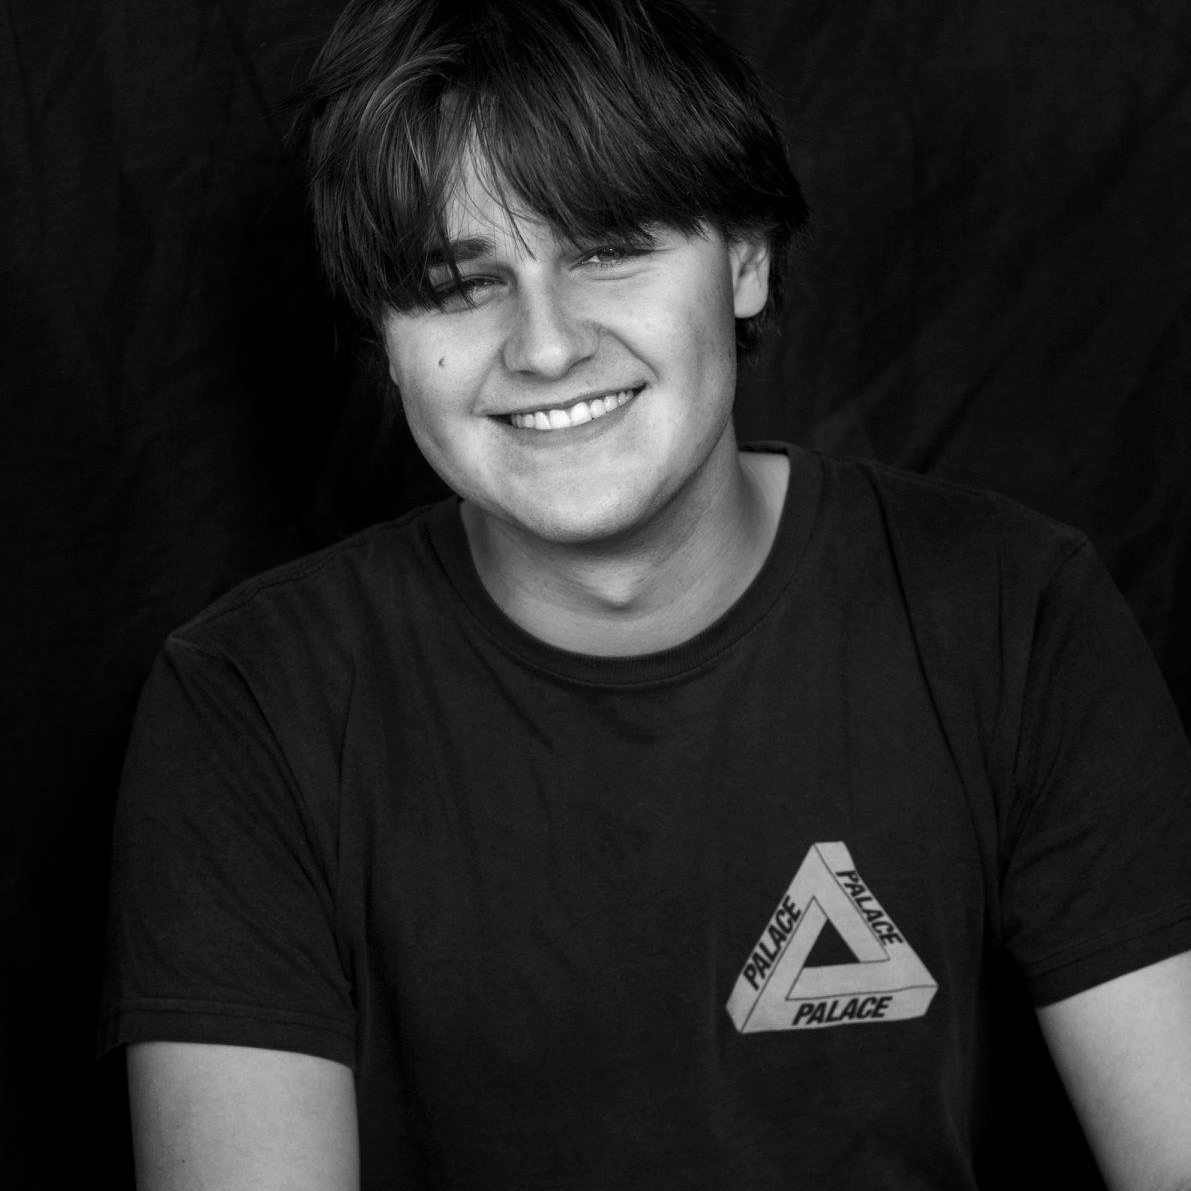
\includegraphics[width=\textwidth]{pb}

\begin{center}
	\large\textbf{Introduktion}
\end{center}

Et orblindt individ, ved navn Andreas, har begivet sig ud i at fortælle fortællinger. Fortællinger, der forhåbentligt underholder. Fortællinger, der forhåbentligt giver dig lyst til mere. Relationer til det ukendte og overnaturlige. Relationer mellem mennesker. Relationer mellem verdner. \newline
Du er opfordres til at begynde, ved den fortælling, der tiltaler netop dig mest.

\newpage

\begin{center}
	\LARGE\textbf{Indholdsfortegnelse}
\end{center}

\section{I - 3}

\section{En mand der finder indhold i livet - 7}

\section{A True Mystery, Indeed - 17}

\section{Svenska korvrätt - 24}

\section{Meddyusas indflydelse - 29}

\section{Hvor er mor?}

\section{Lies and Snake-Eyes}

\section{Drømmenes mysterier}

\section{The Goddess Child}

\section{A cup of water}

\section{Hjon}

\section{Kære dagbog}

\section{The Demon Hunter and Spirit Savior}

\section{Sikke en dag}

\section{Manden der kunne modstå}

\section{Svenska korvrätt - Dansk version}

\newpage

\begin{center}
	\Large\textbf{I}
\end{center}

\begin{center}
	\large\textbf{1. I}
\end{center}

To whom it may concern, for those willing to listen and the few, who has nothing better to do, i'd like to tell a story. The whole ordeal started an early morning, just about 7 a.m.I noticed nothing strange, as I got out of bed. It was a small bedroom, with just enough place for me to work, thorughout the day. After booting up my computer, so it would be ready for later, I went to the kitchen. The kitchen is small, with just enough room for one man, but that's okay. I always cook. I always start my morning making the same discount coffe. It makes the early day easier. 
\\ \\
With the coffe in my hand, i go to the bathroom. The coffe also makes this easier. Flush out the body, and the events of the preivous day. For my next ritual, I wander in to the livingroom, trying collecet the last pieces of myself, so the day can finally start. I always end up sitting in the same chair. A comfy chair no one ever really uses, since it isn't that comfortable. But once it was all I had. So I'm used to it, and it had a nostalgic feeling to it. I slowly wake up. It's going better than normal, better than expected. Yesterday was a late night.

\begin{center}
	\large\textbf{2. She and I}
\end{center}

She didn't even notice me, when I arrived home, late at night. I, however, notice the cliking sound. The noice from the bedroom. The commotion she likes to wake up to. I am mildly annoyed. She was a black magic woman, with bleached hair. Her lips was big, lovely for a kiss, amongst other things. Her cheaks was round like an apple. She had shapes, like a natural woman. A bit extra kilos, but that never bothered me. Her eyes were brown, but they never really captured my attention. I never got lost in them. 
\\ \\
As I sit there, and think of her, my mind starts to wander, as the noicy cliking  becomes a meditative inspiration, instead of an annoyance. My eyes wander through the room, as I notice things I have never noticed before. A black spot on the ceiling right by the corner. A red light from the sun, on an ugly painting of a human being, my mother gave me. A dying plant, beyond saving. A few cobwebs, dangling around. The dust became noticeable, because of the sun. A letter on the table, I inherited from my grandfather. I start to become a part of the room, as the clicking goes on. My sense of being disappears. 
\\ \\
The clicking stops. I start to exist again. I started to wonder about the letter. I move towards the table. I look in the letter. It's from her. It's over. Almost soundless I whisper "It can't be real, wake up", as im softly wacking myself, with a banana, that was lying in the fruit ball she made. It was the only thing of hers in the apartment. She could take ownership of it all, it wouldn't matter. All I want is the love of my life to come back, so I can see her one last time. So I can say goodbye. So we can part ways in a proper way. Next to the letter there is a carving. It says "I loved you. Never forget that".

\begin{center}
	\large\textbf{3. Her, She and I}
\end{center}

Days have passed, and I can't seem to get myself out of my head. I can't take it anymore. I go to the local pub, to do the one thing, i promised myself not to do: Buy one pint. One pint, that leads to another. The spiral starts. I've been to the pub pleanty of times before, but never alone. Being alone at a pub is a dangoures game. You, alone with only the alcohol. You, alone with your own thoughs, that get worse and worse for each sip, you let through your body. And a cat that the pub has claimed ownership of. 
\\ \\
A women with a stripe on here face, starts singing in the back of the room, as she slowly dances, with out my knowlagde, closer and closer, sexy as can be seducing every man in the room. I light a cigarette, even though I already have one. It's almost done, I say to my self, and my glance becomes split, as I for a shot moment see it as 4 ciggarets lying next to eachother. 
\\ \\
The woman is comming closer, and I start to notice her singing. I suits me. I slowly move in a 180 degrees movement, and smell a fragrance so delightful, it cancels out all my other senses, for a shot moment. I see her. my senses are again canceled out, by the sight of her. She's standing there. A completly pale body, that hasn't seen sunlight in ages. Black hair, that incapters the light, and gives of a special glow. Her essence is sexy, but yet so classy. Her eyes. Oh her eyes. Soft, smiling but yet direkt and cold. Like an ocean, where a sailer could get lost, but somewhere, out there, something is worth dying for. Her mouth was smiling, like there where a seacret on her lips. A soft smile. But a trained one, that can be givin even at a funeral. Her face collects all of her facial expressions in to one. 
\\ \\
I don't remember her body at all, maybe beacuse of the alcohol or maybe because of her captivating face. This woman has already forfilled my needs, with just a song, and a mesmerising stribed face. What a woman.

\begin{center}
	\large\textbf{4. Them, Her, She and I}
\end{center}

As I sit at the bar talking, while she's sitting there listening, my mind slowly forgets about my loved one, as the monolog becomes more and more about my passion than my sorrow, as im slurping my way through pints upon pints. It is like the only sense I have, is the ability to talk. I have a connection with this human being, that I have never experienced before. After awhile, she surgests a change of surroundings. I agree instantly. Where ever she wants to go. 
\\ \\
We walk through the town. The town is like any other. Shops, pubs, and streetlights. As we walk in the cold winter wheather, with new snow slowly faling beautifully from the sky, and laying atop of the roads as a blanket, she starts to sing. A spellbinding song. A song of a siren. I can't think or talk or see. I can only listen, as all my other senses slowly fades away. My body goes to autopilot. I just walk, and she leads me with her voice. 
\\ \\
She stops singing. We stop. I start existing again. It's a hosue. The house is painted with graffiti. Waves, splassing togehter and boats cracking, sinking into the deapths of the unknown water. There is a piece of wood, from what appears to be from an old boat. The piece of wood tells me, that the house is called Odysseen. She takes me inside. The song that she is singing, becomes plural. The voices brings me into the livingroom, where there are anchors, rudders and ropes on the walls and a small fireplace crackles a rythem, as the clicking noise, from her bedroom. 
\\ \\
There are 13 women, all singing and slowly dancing. They all have the same captivating glance in there eyes, as the woman who lead me here. They all have the same pale color of skin, black hair and a stripe on their face. They all look so different, and yet, so alike. They place me in a chair. So comfortable. I have never experienced something like it. They gather around me, still singing and dancing. Slowly they start touching, caressing and massaging me. I close my eyes, and my sense of touch slowly returns. This must be heaven.

\begin{center}
	\large\textbf{5. You, Them Her, She and I}
\end{center}

Some bealive that before you go to hell, you need first to experience heaven, so you know the difference between the two. So you know you have it better or worse. As I sit there, slowly drifting to a dream state, becoming one with the room. They stop singing. The song has endend. They drag me out of the chair, as it was like I couldn't move. I can't move. I can stand, but my body is numb. 
\\ \\
I start thinking of her. I start to miss her again. Sorrow fills my eyes. The 13 women look at the woman who lead me here, with a disappointing look in their faces. It's the same face she gave me, the night before she left. I hold my head clear. I don't know what's going on anymore. Or where I am. I slowly start to go crazy. I feel like going, but I still can't move. They start singing again. I try to fight it, but the trance slowly starts to come back. 
\\ \\
I'm one with the room. I'm an object. I can move again, but only where and when they want to move me. They feed me with food. The best tasting food I've ever tried. My tastebuds overtakes my body. I only sense the bits danicing on my tongue. They strip me down, from top to tow. I let them. As a sexual journy is about to begin, they stop singing again. The sexual experience is soundless. It's amazing. With closed eyes, it becomes so intence. They stop. For a short while, im back, wondering what is going to happen. They start singing again. 
\\ \\
I am in their power. They move me outside. Through the streets. There isn't soul in our path. There are no lights in any of the houses. The lights from the sky, is so pleasent, like the sun is shining in the darkness. It has stoped snowing. Every footstep I take, should ruin the beautifull snow blanket. But nothing happens. The snow stays intakt. We get closer to the towns river. On the river there is a flume floating. Nothing but the flume. We board the flume. The water was frozen. The flume was stuck. The singing intensified. I am now free. Free to move. But I don't want to get off the flume. It's like im keeping myself in captivity. 
\\ \\
As I stand on the very eadge of the flume, looking at the ice, it slowly starts to melt. It seems as if the song is making the ice melt. Slowly a hole is forming. A hole in the ice. They finish what they started in the bed. Again soundless. As im stiped naked, I suddenly I start walking slowly thowards the hole in the ice, without resisting, just moving slowly. I jump in. It's warm, comforting yet terrifying. The singing stops. I see the women leaving. I try to swim, but my movement hasn't come back. Im drowning. Suddenly a hand appers. It grabs me, and pulls me out of the water. It is you.

\newpage

\begin{center}
	\Large\textbf{En mand der finder indhold i livet}
\end{center}

\begin{center}
	\large\textbf{1. Aarhus’ Å}
\end{center}

Jeg kom gaående igennem en gyde, midt I Aarhus by. Der lugtede af pis. Klokken var efterhånden blevet mange og sommerens dunkle lys, havde stille lagt sig, i byens ellers så oplyste gader. Grafittien på væggene vekslede mellem en dårligt Tegnet penis, til storslået kunstværker, nogle gange med en penis på. Min mor havde beordret mig at tage en ekstra trøje på. Selvom min alder ellers er oppe i tyverne. Set i retroperspektiv, er jeg glad for min mors insisteren. Den kolde kulde giver anledning til kuldegysninger og gåsehud.
\\ \\
Selvom mørket havde lagt sig, kulden gav kuldskær og gadelygternes lys sad lige i øjenene, var jeg glad for den udendørs vandring, jeg havde begivet mig ud på. Mine tanker racede afsted, med en vis hastighed. Det var begyndt at ske oftere. Tanker der gerne gør mig istand til at forstille at guds plan for mig, må være ligeså storartet som Einstein eller Jesus. Tankerne var og er stadig, ikke altid direkte og rationelle. Manisk.
\\ \\
Jeg havde været hjemme hos en af mine bekendte. Kløgtige Mads, som
vi plejede at kalde ham. Lidt ironisk, da Mads’ kløgtighed ikke kunne måles med resten af slænget. Dette er jeg ikke sikker på at han ved. Det er sikkert også for det bedste.
\\ \\
Hans lejlighed var noget sølle, med et badeværelse ved siden af køkkenet. Begge rum med dårlig udsugning. Den hærlige lugt af kattofler i ovnen, blandet med den hæslige lugt fra de udskylde oppusted kattofler. Han bruger sit værelse, på ca. ni kvadratmeter (otte, men i den høje ende, hvis man overvejer kommatalende). Der er lige plads til hans skærmfetish, tre på skrivebordet, og et TV på en lille reol, en reol til, en seng, enmands da han er single, en kommode og en sofa en ret god sofa. Hvordan kløgtige Mads har skabt plads til alt dette, må kun guderne vide. Eller måske er det muligt, at alt den tetris han valgte at spille i folkeskolen, endelig har givet ham en fordel i livet.
\\ \\
Byvandringen har ledt mig ned til Arhus’å. Dette er punktet, hvori forståelsen for, hvorfor denne nat sidder indprintet i mit hoved. En af de få gange, hvor man kan være sikker på at printeren altid virker. Der lå en i åen. Spørgsmålet var, og er på sin vis stadig i dag, hvad jeg kunne gøre ved netop dette. Mens jeg ringer et-et-to, overvejer jeg hvor smart det ville være, både æstetisk og praktisk, hvis man kunne have en paraply og en fiskestang i én. Så kunne jeg blot fiske vedkommende op. Hvis jeg da ellers havde en paraply. Hvis jeg da havde et mod til døds fiskeri.
\\ \\
Der kom en kranbil. En forvokset fiskesang, hvis du spørger mig. Der dog også kan bruges, i terræn der ikke er vand. Dog manglende en paraply. De hiver vedkommende op af vandet, mens en rar mand kaldet Niels, står og udspørger mig om diverse ting. Det er rart. Det er ikke så ofte folk spørger ind til min dag. Så udluftningen af dagens forløb, bliver lidt mere detalieret. Men det virker som om Niels er glad for det. Sikke en hærlig mand.
\\ \\
Det er en kvinde. Et kønt stykke kvinde køn. Hvis man ser bort fra vandets hærdning og dets ellers så renlige affald. Hendes hud var smuk og blej. Formentlig grundet den grundige fermatering vandet havde udøvet. Sort hår. Knald sort. En fantastisk kontrast til hendes smukke hud. Det var svært at se ansigtet, men det lignede at hun havde striper, en form for ar, ned over ansigtet over det hele. Et meget gustent syn. Tøjet sagde mig ikke meget, men jeg er jo hellere ikke modeansvarlig. Det er trist man ikke kan se hendes øjne.
\\ \\
Det er nu, efter den grundige analyse af liget, at hammeren falder. Chocket slår til. Jeg besvimer. Og vågner. På et hospital. Sikker noget. Sikke en aften. En oplevelse for livet, bør porienteres.


\begin{center}
	\large\textbf{1. Aarhus' Åndsbolle}
\end{center}

Jeg har hjernerystelse. Jeg ligger på hospitaltet. Uden busker på. Jeg vågner simpelthen op, i en fremmede seng uden bukser på, mens en flot pige kommer med morgenmad, og spørger om jeg har sovet godt. Det er sku aldrig skeet for mig før. Jeg er ør i hovedet, og formulere et elendigt svar. "Jaja, helt sikkert der, det var sku ok, jeg var helt væk." Fuck mig. Hun er høffelig. Det følger vel med til jobbet. Hun går. Jeg putter pænt min serviet fast i blusen, i tilfælde af at jeg skulle spilde. Jeg spiser roligt min havregrød. Bedere end forventet. Jeg drikker glasset med juice i en tår. Ja, tørsten var sku stor.
\\ \\
Rummet var sterilt. Hvide væge. Hvide senge. Vidt over alt. Sågar en hvid sengekammerat. Der er dog et billede på vægen. Det er af en strand. En hvd strand. Med hvide mennesker der går på den. Blåt hav, men hvide skyer. Der kom en mand i hvid kittel og sagde "Du må godt gå nu!" med lidt irretation i stemmen. Så jeg tog mit tøj på. Der kom lidt farver på værelset i et kort øjeblik, før jeg gik ud af døren.
\\ \\
Det blev morgen. Eller, klokken slå fjorten. Jeg vågnede. Tog min morgenkåbe på og gik ud i køkkenet. Lavede 2 spejlæg. Med timina, salt og peber. Jeg gik ind på mit værelse. I mørke. Mørklægningsgardinerne blev ikke trukket fra. Solen havde ingen plads på værelset. Jeg tændte op for et afsnit "Friends". Sæson 3, Episode 3. "The One With The Jam". I en tidligere episode, havde Richard og Monica slået op. Grunden til dette var, at Richard ikke ville have børn, mens Monica gerne ville. De så derfor ingen fremtid i forholdet. I episoden lige før Episode 3, prøver Ross, at få slænget til at gøre sig klar, til en vigtig begivenhed på museet, hvor han arbejder. Både Chandler og Joey drikker fra et glass fyldt med fedt, i troen om at det er cider. Monica er ikke særlig glad for dette. Gad vide, hvad hun skulle bruge et glas fedt til?
\\ \\
Det hele starter med, at Chandler sidder og læser en bog. Vi for ikke oplyst, hvad bogen handler om. Der kommer nogle knirke lyder, fra en seng, inde fra Joey's værelse. Her tænker man straks, at han elsker med en kvinde. Vi hører et skrig, og finder ud af at Joey hoppede i sengen, og da faldt ned. Chandler siger "See, Joe, that's why your parents told you not to jump on the bed." En fantastisk start. Den holder virklig ens interesse.
\\ \\
Vi bliver intruduceret til afsnittet, ved at Monica laver "Jam" fordi, hun er deprimeret over Richard. Hele slænget kommer und, undtage Phoebe. Joey er vild med "Jam". Han smager på lidt direkte fra gryden, men det er for varmt. han ender med at spytte det tilbage i gryden. Ha, klassisk Joey. Joeys arm også kommet til skade med sin arm, da han faldt ned fra sengen. 
\\ \\
I den næste scene, ser vi Phoebe blive forfuldt af mand. Men han tror det er hendes søster, Ursula, som han datede i lidt tid. Han stalker altså den forkeret søster. Phoebe tilgiver ham. Hun giver rådet "You are not a witch, you are just an avarege student" til stalkeren. Hun ender med at invitere ham på kaffe.
\\ \\
Rahcel og Ross kommer op i den lilla lejlighed, hvor de opdager at de er alene i lejlighede. De "hygger" lidt. Men Chandler kommer ind, stopper dit brat. Han har et problem med sin kæreste "Janice". Jeg vil ikke gå formeget i dybden med problemet. Det må være en lille teaser til dig som læser, så du selv kan se episoden, og stadig have nogle overraskelser. Dem skal jeg nok lave lidt flere af ;)
\\ \\
Vi befinder os nu på caféen "Central Perk" hvor joey sidder op putter, he, lidt for meget, kan man vel sige, syltetøj på en scone, tror jeg. En eller anden type bolle, i hvert fald. Hele slænget er det, ud over Phoebe og Monica. Phoebe kommer dog ind, og slutter sig til gruppen. Hun fortæller om sit møde med sin stalker "Malcome". Joey sige, he, han er sku sjov, han siger "You talked to him?" mens hans mund er helt fyldt med bolle. Der er krummer ud over det hele. Monica joiner da festen, så nu er de alle samlet. Chandler spiller spørgsmålet "Det girl from det xerox place, buck naked, or a tub big of jam?" og Joey, sjov som han er, siger "Put your hands together" Haha, den for mig vær eneste gang jeg ser afsnittet. Monica fortæller om sin nye plan, for at komme over Richard. Babyer. Via en sæd donor.
\\ \\
Chandler oplever de samme problemer, men har nu en løsning fra Ross. Men igen, se du det selv. Så er det lidt mere spændende. Phoebe ses hvor hun hjælper stalkeren "Malcome". Men det må du også selv se, jeg vil ikke røbe for meget
\\ \\
Monica mener hun har fundet sin perfekte sperm donor. De andre taler imod idéen. Men hun forsvar det. Joey laver "Jam crackers". Han er altså hyle morsom. Hun finder Joey, som sæd donor. Phoebe foræller om hendes møde med Malcome, og så kommer en scene med Chandlers problemer, og igen Phobe's. Igen, det må du selv se, din bavian. Det er et godt afsnit.
\\ \\
Moica har valgt sin donor. Hun snakker med lidt med Joey omkring det. Han fortæller om hvordan han ville have set hendes fremtid, yderligere med hendes fremtidige mand. Han forstiller sig at de har skilt, hvor der står "We don't swm in your toilet, so don't pee in our pool." Ha, som om det ville stoppe mig. Han fortæeller om deres fælles børn. En dreng og to piger. Samtalen for Monica til at skifte mening. Men bliver lidt ked af det, og som den gode person Joey er, trøster han hende. Sidste scene er omkring Joey, der sidder og snakker om at han der ikke er nogen der har været intresseret i hans sæd. (det vill jeg være, hvis jeg var en kvinde, hehe) Han spiser syltetøj, og for det ud i hele ansigtet. Ross kommer hjem, og Rachel er sur på ham. Det er grunder Chandler situationen, så jeg afslører intet. Så er afsnittet slut.

\begin{center}
	\large\textbf{1. Aarhus' Århusianer Vaner}
\end{center}

Jeg sidder i min sofa. NetFlix har spurgt om jeg stadig ser venner. Det gør jeg ikke. Skærmen går i dvale, og bliver sort. Jeg kigger i det sorte spejl og ser mig selv. Jeg klør mit i skridtet. Jeg finder min mobil frem for at ornanere. Efter jeg er færdig, låser jeg skærmen. Igen, kan jeg se mig selv. Jeg skammer mig. Jeg har ikke lavet andet end at spise æg, se venner og onanere de sidste par dage. Måske jeg skulle se at komme ud af huset. Det er jo sol og sommer.
\\ \\
Jeg er solallergiker. Det vil sige, at i skarpt lys, så som stærk sol, nyser jeg. Denne sommer er det gået helt amok. Nys efter nys efter nys. Min cykel er punkteret. Øv. Det vidste jeg godt. Det gider jeg ikke fikse. Jeg går ned mod bussen. Jeg har glemt mit rejsekort. Øv. Jeg må gå. Jeg kan ikke lide at udnytte den offentlige transport. Det er jo nærmset tyveri at køre uden billet. Gåturen er lang. Eller, for mig er den lang. Den tager godt og vel femogfyrre minutter for de fleste. For mig tager det tres. Jeg er et reflektivt menneske, og elsker at kigge på omverdenen, mens jeg bevæger mig igennem dem.
\\ \\
Jeg går ad store veje, små veje, ved cykelstiger, universitets parken og Ø gade kvarteret. De store veje er et godt blik på Aarhus. Altid stress. Alle skal et eller andet sted hen, hurtigt. På de store veje, har alle ideologien om, at de er de vigtigste og eneste på vejen. De store veje er kun gode, da man må fokusere viljefast på musikken. Musikken leder til tanker. Tanker lede til god tidsfordriv. Jeg høre den samme sang på repeat.
\\ \\
Små veje og cykelstiger er lidt bedre. jeg nyder at se folk i deres hverdag. Fundere over deres liv. prøve at forud se, om de er sent på den, på vej hjem til en fodbold kamp eller skal til fest. Der er altid nogle der skal noget, men modsat de store veje, er folk her observante på hindanden. På dette tidspunkt på dagen, er det dog mest folk der tager det meget afslappet. Det er en rar atmosfære at være i. Det samme er der i universitetsparken. Der er lidt ude og drikke øl. Nogen har en højtaler med. Andre spiller spillet "kævle". 
\\ \\
Det handler om at stå to hold på være sin side. Typisk 3 meter fra midten. I midten står der en kævle. Det gælder nu om at vælte kævlen. Mand har et forsøg. Man kaster med en sko. Rammer man kævlen, så den vælter, skal man drikke af sin øl, der selvfølgelig fra start er fuld. Her gælder det om for det andet hold, at at hente skoen, samt sætte kævlen på plads igen. Nå dette er gjort, skal det andet hold stoppe med at drikke øl. Når alle af holdets øl er tømt, vinder holdet. Sikke et spil.
\\ \\
I parken spilles mange andre drukspil. Det mest velkendte ville vel være "øl bowling". Det er så kendt, at jeg går ud fra at jeg ikke behøves at forklare reglerne. Ellers så brug google. Det er altid rart at vandre i en park. Specielt om sommeren. Specielt denne park. Med alle de studenterrelatered traditioner, så som kapsejladsen. Ja, det er altid rart, selv om vinteren, at vandre i et naturområde med liv, midt i en stressende by.
\\ \\
Ø-gade kvarteret er blot et hyggeligt område. Her bor så mange friske unge mennesker. Lejlighederne er gamle. Rustikke. Forskellige. De er unikke. Alle jeg har kendt, der boede her, har været ekstatiske over at bo her. Og man forstår godt hvorfor. Som jeg sagde om de stille veje, giver man plads til hindanden. Dette er et helt område, hvor folk giver plads til hindanden. Mangfoldighed.
\\ \\
Jeg når ned i latiner kvarteret. Min disination. Mit favorit område. Det er det sted, i byen, hvor jeg føler mig mest hjemme. Mødestedet for mig og mine bekendte. Mødestedet, hvor man drikker kaffe om dagen, og øl om aftenen. Ja, det er her jeg begiver mig hen. Grunden er kaffe. Jeg ville ønske jeg havde en i mit liv, der ville drikke en med mig, men dette må blive en anden gang. Denne gang er det mig, kaffen og cigaretten. "En kop kaffe, gerne så sort som sjælen selv" siger jeg selvsikkert, mens jeg fyre op for et søm. Et søm, der stille bankes i kisten.

\begin{center}
	\large\textbf{1. Aarhus' Ånd}
\end{center}

Jeg sidder nu på min favorit café. Jeg kan lide den, fordi musikken er god, dog i sådan en volummen, der gør at man stadig kan høre hvad der sker. Jeg sidder ved et bord. Et tomands bord, hvor der faktisk godt kan sidde fem. Jeg skodder min cigaret. Tænder en ny en. Inhalation. Ekshalation. Inhalation. Ekshalation. Sug ind. Pust ud. Det kunne næsten lyde som om, en jordmorder var ved at lære mig at ryge.
\\ \\
Mens jeg sidder og lytter til samtalerne der er omkring mig, da de er meget mere indholdsrige end mit liv. Lidt mere spændende end binging Friends. Ved sidden af mig, er der en ung pige. Hun har problemer med sit sex liv. Hendes dating partner fra tinder holder for længe i sengen. Hun fortæller, at det varer mindst tredve minutter. Ofte længere. Hun keder sig under sex og hendes nedre dele er begyndt at gøre ondt. Rigtig ondt. Hendes veninde forslår, om det kan være at det er fordi han ikke tænder nok på hende. De griner begge to. Deres næste samtale er ikke spændende, så jeg bevæger satelitten til nye lydbølger. 
\\ \\
Der er et andet spændende par. Deres samtale går meget langsomt. Ganskevist fordi de spiller skak. Dette gør samtalen, eller i hvert fald situationen, meget mere spændende. Selvom de ikke er særlig gode. Jeg har lyst til at hoppe ind, hele tiden, og give dem det oplagte træk. De kan jo tydeligvis ikke finde ud af det. De er slet ikke på mit niveau.
\\ \\
Efter at have skandet rummet med mine satelliter, må andres liv skuffe, da de giver mig mere lyst til at se Friends. Hold kæft hvor blev folk kedelige. Fuck dine studieproblemer. Jeg går på toilet. Toiletet har altid været et af mine ynglingssteder på caféen. På vægene er der ophængt gamle reklamer, med alt fra rengørningsmiddel, arnbitter og knorr bearnaise sovs. Selve toliet er rent. Ligeså vasken. Det sætter jeg pris på. Håndtørren irritere mig. Mine hænder bliver fandme aldrig tørrer. Men for at gøre det fair, så har jeg aldrig oplevet at nogen håndtørrer har virket ordentligt. Så det ser jeg bort fra.
\\ \\
Da jeg kommer tilbage fra toillet, sider der en kvinde ved mit bor. Bleg. Hendes hår var uglet. Hendes krop var bleg. Grønlig. Det lignede næsten at den var fermenterede. Havde en speciel udstråling. En gylden udstråling. En bleg gylden udståling. Hun var smuk. Uffateligt smuk. De samme striper i ansigtet som kvinden i åen. Hun sad og sang, med på teksterne musikken spillede. Hun sang højt. Men det var som om ingen lagde mærke til det. Det var som om ingen kunne høre det. Det var som om hun kun eksisterede i mine øjne.
\\ \\
Jeg gik op i baren for at købe en frisk kop kaffe. Da jeg kom tilbage og satte mig, kunne jeg se at der var to glas chartreuse. Med isterninger. Hun stoppede med at synge. "Hello Sir" sagde hun til mig. Med en sexet stemme. "My name is Meddyusa" forsatte hun. Hun tog en tår af sit glas chartreuse. Hun hentydede til, at jeg også skulle. Jeg var forundret. Facineret. Nysgerrig. Så jeg tog en tår. Det brændte og smagte ikke som det plejer at gøre.

\begin{center}
	\large\textbf{1. Aarhus' Åndsmenneske}
\end{center}

"Why are you here?" Jeg forsatte, mens jeg satte drinken ned. "What is you agenda?" Jeg tog en ciggeret og smed den i munden. "How rude of you not to present yourself." sagde hun med en vrissen tone i stemmen. Jeg kunne godt se, at jeg lige var lidt uhøffelig og skyndte mig straks med at svare. "Adam ." og jeg fortsatte "Would you know please awnser my question?" sagde jeg lidt irriteret. "You seem lonely. So I thought I would keep yor company." 
\\ \\
Hun begyndte at stille nogle personlige spørgsmål. "Have you erver found a woman, you could could and would keep in your life?" Et aggresivt spørsmål. Et spørgsmål jeg ikke helt vidste hvad jeg skulle svare på. Jeg havde aldrig haft det. Kun små flirts, hvor pigen gav op på mig. Det er det jeg må sige. "No, I haven't." sagde jeg med generthed i stemmen. "I guess you just never met the right one. One to keep you in check." sagde hun. Hun ville gerne høre mere om det. "I think I never found anyone that complement me. I guess nobody see's me as the right one." "Have you ever had sex?" she said, with a wink and a smile. "No. No i haven't. I'm fairly good at talking with girls, but it's never been more than a kiss."
\\ \\
Samtalen forsatte på denne måde et kort stykke tid. Men så begyndte hun at stille mig spørgsmål om mig. Om hvad jeg havde af hobbier. Hun lod mig tale. Når jeg taler reflektere jeg. Så det jeg ville sige, kørte altid over i noget andet. Hun lod mig bare tale. Dialogen blev til en monolog. Omkring mit liv. Omkring mine skader. Både fysisk og psykisk. Det var rart at have en som lyttede. Efter noget tid, spurgte hun, om vi ikke kunne gå et mere stille sted hen. Jeg tog hende med i parken. monologen forsatte. Lidt endnu. Så forslog hun, om vi ikke skulle tage hjem til mig. Jeg afviste. Jeg løj om at jeg blev nødt til at gå. Hun lagde op til sex. Min nervøsitet vedrørende sex var for stor.  Jeg kunne ikke håndtere det. Jeg forlod hende i parken. Hun virkede ikke glad. Hendes udstråling gik over, og blev mere aggresiv og fjendtligt. Hendes skær gik stille fra blåligt til blod rødt.

\begin{center}
	\large\textbf{1. Aarhus' Ånds Åndedrag, mit Åndedrætsbesvær}
\end{center}

Jeg tog en bus hjem. jeg var lidt i chock. Det var som om hun aldrig var blevet afvist før. Jeg følte mig træt i kroppen. Som om der havde været en besværgelse, der havde forsøgt at overtage min krop. Busturen er kun ti minutter lang. herefter skal man gå i fem-ti minutter. Alt afhængigt af om lyskrydset er grønt, og hvor hurtigt man går. Mine ben var stadig gummi. Så det tog faktisk et kvarter denne gang. Da jeg kom hjem, var min roomie ved at lave mad. Den gode paprika gryde, han laver mindst en gang om ugen.
\\ \\
"Så kunne du fandme være hjemme, hva' Adam. Det er jo lige før du ikke nåede maden." sagde han, med et smil på læben. "Nu skal du fandme høre hvad der skete for mig, makker." Jeg fortalte historien, over paprika gryden. *smask* *smask* "Og så tog vi i parken, og..." blev jeg ved. Men i kender jo historien, så jeg vil ikke gentage. "Kæft man det lyder sygt homie. Men hvorfor fanden tog du hende ikke med hjem? Det er jo gratis fisse lige der, homie. Det er sku da på tide, at du for parkeret bilen i garagen." 
\\ \\
Han havde en pointe. "Hvor meget bliver maden, Karsten?" sagde jeg, for at skifte emne. "Kun 13 kroner i dag du. Kødet var på min mors regning." sagde han med stolthed i stemmen. Det var også imponerende billigt. "Jeg har sendt på mobilepay" sagde jeg, mens jeg begyndte at tage af bordet. Den ene laver mad, den anden tager opvasken. Det er aftalen. Der var heldigvis ikke så meget, og så har vi en opvaske maskine. Så man skal ikke stå med tallerknerne. Det skulle jeg i min gamle lejlighed. Det var et heleved. Specielt når der havde været gæster.
\\ \\
Men jeg stod og dansede til den gentagende lyd af "New Drug" med Jinji Kikko, var det som om noget pludselig ånede mig i nakken. En kold ånde. Kort men skræmmende. "Det var sikkert bare lidt gennemtræk" tænkte jeg for mig selv. Det skete igen. Der var ingen døre eller vinduer åbne. Det var jo lidt koldt udenfor. Hvad fanden, tænkte jeg. Det skete ikke igen. Før morgenen efter.
\\ \\
jeg stod i badet. Hørte "Sexual Healing" af Marvin Gaye, på fuld skrald. Jeg sang med, godt nok i lav volummen, så Karsten ikke kunne høre det. Det skete igen. Mens jeg stod i badet. Denne gang voldsomt. Så voldsomt, at jeg næsten faldt. Jeg skyndte mig ud af badet. hele rummet var dampet. Jeg kan godt lide varme bade. Håndkldet blev smidt rundt på kroppen. Jeg var stadig våd på ryggen. Jeg gik ud af værelset, og fandt mine angst piller. Rivotril. Mand må tage tre om dagen. Jeg tog alle på samme tid. Jeg sad i ti minutter, klamret sammen i fosterstilling. Pillerne virkede endelig. Jeg kunne slappe af. Puha, sikke en oplevelse. 
\\ \\
Ånden blev ved. Jeg var så skræmt. Jeg kunne næsten ikke trække været. Jeg hørte døren smække. Karsten skulle på Uni. Det gjorde det ikke meget bedre at jeg var alene. jeg var lige ved at ringe til læge vagten. Man skal igennem læge vagten før man kan komme til psykiatrisk vudering. Da jeg havde tastede 5 ud af de 8 tal, bankede det på døren. Jeg gik ud og åbnede. Jeg kunne ikke lade vær. Det var som om noget styrede mig.

\begin{center}
	\large\textbf{1. Aarhus' Åndelig sang}
\end{center}

Der stod en kvinde. Et smukt eksemplar af en kvinde. Hun havde nogle træk ligende kvinden fra åen, dog var hun sin helt egen. Hun havde en del make-up på, men inden bagved kunne mand se en stribe. Det lignede næsten et ar. Hendes hår var langt, glat og blond. Det var så langt, at det gik helt ned til røven. Gad vide om hun nogensinde, er kommet til at skide lidt på sit hår? En finurlig lille tanke. Dem er vi glade for. Hendes krop var kurved. Hendes hud var mørk i det. Ikke sådan mulat/sort, men nærmere som en bleg krop som var lidt solbrændt. Hendes tøj var lidt slattent. Det passede ikke helt til hendes kropslige udstråling. Men som pointeret tidligere, har jeg ikke forstand på mode. Jeg vil derfor ikke kommentere mere på valget af tøj.
\\ \\
Mens jeg stod og beundrede det smukke syn, med elevatorblikke, der kørte op og ned, fra første sal, til tagterrassen og ned igen, stod hun og sang. En smuk sang. Det var dog lidt mærkeligt. Mit syn gik fra beundrende til små irriteret. "Hov, altså undskyld mig, men hvad er det du laver her, om jeg må spørge?" afbrød jeg hende, midt i hendes ellers fine sang. Hun så forvirret ud. Hun stod bare og kiggede lidt på mig. Så var det som om, hun kunne høre en stemme. Lidt alle det udtryk, en vært for, når vedkommendes producer fortæller dem noget i deres øresnegl.
\\ \\
"Må jeg få en kop kaffe?" spurgte hun "Jeg bor i området og har set dig gå ture. Du ser så sød ud, at jeg bare måtte have en snak med dig!" Lidt mærkeligt i mit syn, men jeg var aldrig blevet beundret før, i hvert fald ikke hvad jeg ved af, så lidt i chock gav jeg lov. Heldigvis er jeg lidt af en kaffe narkoman, så kaffen var allerede klar og varm. Jeg hældte en kop op til hende. spurgte om hendes navn. Det var Eva. Sikke et finurligt navn, når man nu overvejer mit. Adam og Eva. Begyndelsen på noget nyt. Begyndelsen på paradis. Jeg må bare holde hende fra æblet. "Vil du ikke med ind på mit værelse? Der er så mørkt i stuen" forslog jeg. "Det lyder bare godt." sagde hun næsten, før min sætning var færdig. Vi sad nu og snakkede lidt frem og tilbage. Men dialogen blev hurtigt til en monolog. Hun ville høre om mit kærligheds liv til at starte med. Det undrede mig.
\\ \\
Både pigen på caféen ville høre om mit kærlighedsliv, og nu denne skønne pige. Men siden hun havde beundret mig en smulle, giver det vel fin mening, at hun gerne vil høre om der kunne være en mulighed, for at skabe et forhold mellem os to. Så samtalen gik meget, som den på caféen. Monolisk. Fra kærlighed til hobby og hverdags liv. Jeg fik lov til bare at plapre løs. Det var faktisk lidt kedeligt. Så jeg beyndte at spørge ind til hende. "Hvordan er din hverdag så?" 
\\ \\
Hun så igen forvirret ud. Som om hun havde regnet med, at jeg bare ville plapre videre om mig selv. "Det er da kun høfligt, at spørge ind til vedkommendes liv." sagde jeg, med et smil på læben. "Ja, ja det har du ret i!" sagde hun, mens det igen lignede, at hun fik en besked i øret. "Jeg arbejder lige nu. I et sushi sted. Så kan jeg få billig sushi." forklarede hun. Hun fortalte videre. Ja sagde engang imellem "Ja" "Aha" "Spæendende" osv. Bare for at vise, at jeg altså hørte hvad hun sagde. Hun virkede mere naturlig og afslappet nu. Hun drak ikke af sin kaffe. "Hvordan kan det være, du ikke drikker af din kaffe?" spurgte jeg undrende. "jeg kan faktisk ikke lide kaffe. Det var bare en undskyldning for at snakke med dig." "Hvad med the? Kune det interessere?" "Ja, ja det ville være fint." Så jeg lavede noget the.
\\ \\
Men pludselig blev hun stiv. "Skal vi have sex?" sagde hun. Jeg var forbløffet. "Hvad fanden er det for et spørgsmål? Sex er en intim aktivitet. Det er altså ikke noget man bare skal gå rundt og tilbyde, bare fordi man har fået en kop the. Nej, du kan få en date med mig, det er det du kan få! sagde jeg med hidsighed i stemmen. Hovedsageligt fordi jeg var bange for sex. hvad nu hvis jeg ikke gjorde det ordentligt. Ville hun så aldrig ses med mig igen? Jeg kender slet ikke til den verden. Den er skræmmende! Hun så lidt skræmt ud. Men takkede ja. Hun ville gerne ses med mig igen. Jeg fik hendes facebook. Så kunne jeg bare skrive, når jeg fik tid. 

\begin{center}
	\large\textbf{1. Aarhus' Ånds Sammensvorne}
\end{center}

Der gik en lille uge, før vi så hindanden igen. Denne gang på min favorit cafe. Vi sås igen og igen. Nogle gange fortæk vi, at komme steder der var velkendte. Andre gange var det spændende at udforske nye steder. Vi gik mange ture. Langs åen, ned til vandet, ud forbi Aarhus Ø. op i botanisk have. Vi sad hjemme hos mig, til tider. Jeg fik dog aldrig lov til at se hvor hun boede. Efter vi havde setes en seks syv gange. Vi var alene hjemme hos mig. Jeg tog fat i mine nossere, og klæmte til. Billedeligt talt. Jeg kyssede hende. På hendes kind. Hun kyssede mig på munden. Det var magisk. Men der skete noget ved hendes udseende. Hele hendes kropsbygning ændrede sig. Mere kurvet. Hendes hør, begyndte at bølge og blive rødligt. Hendes hudfarve blev lidt mere vinter agtig. Hendes ansigt fik lidt mere æble kinder. "Jeg tror jeg elsker dig Adam" sagde hun. Så begyndte hun at græde, og løb ud af huset. 
\\ \\
Jeg kunne ikke få fat på hende. Jeg skrev og ringede firetyve-syv. Jeg bekymrede mig om hende. Hvad nu hvis der var sket hende noget. Der gik en lille uge. Så fik jeg en besked. "Undskyld" stod der. Jeg var forbløffet. Undskyld for hvad mon? Jeg skrev "Undskyld for hvad dog?" "Bare undskyld. Jeg er slet ikke den du tror." Hmmmmmmmm, hvad? "Kan vi mødes. Så kan du forklare. Uanset hvad det måtte være, er jeg sikker på at vi kan komme igennem det sammen." Hun godtog. Vi mødtes på caféen. "Hva' er det så der sker, min kære Eva." Hun var lige ved at begynde at fortælle, førr jeg blev nødt til at afbyde. "Forresten. Jeg har tænkt over det. Og jeg elsker altså også dig. Det troede jeg aldrig jeg ville få sagt. Men det gør jeg altså."
\\ \\
Hun begyndte at græde lidt igen. Med et smil på munden. "Adam. Jeg har været hjemsøgt af en demon. En ånd, der ville have hævn over dig. Hævn, fordi du øædelagde hendes søvn. En kvinde, der var druknet i åen. Hun siger, at hun er dronningen over sirener. Hun overtalte mig til at forføre dig, for at ødelægge dit hjerte. Men jeg kan ikke gøre det." sagde hun, med alvor i stemmen. "Aha. Syret. Okay. Jeg tror lige jeg skal processere det." Der gik lige to minutter, mens jeg sad i Grublerens positur. "Hvad med alt det du har fortalt mig? Er det så også løgn? Fordi det ville nok være det værste. Det ville betyde, at jeg ville have forelsket mig i den forkerte." sagde jeg med bekymring i stemmen. "Nej. Jeg har talt ud fra mig selv. Så vidt jeg ved, er grunden til hun har valgt mig, at jeg er det perfekte match til dig. Så jeg har skullet være ærlig, for at indfange dig. Men efter jeg udtrykkede min kærlighed til dig, har jeg ikke hørt fra hende siden. Det er som om hun er forsvundet."
\\ \\
Vi snakkede længe om det. Men det skulle ikke betyde noget. Hvis du hun havde sagt, var sandt, havde jeg forelsket mig i den rigtige. Også selvom hun måske havde fået lidt hjælp. Jeg kyssede hende igen. "Kom med hjem til mig!" Sagde hun. "Okay." sagde jeg. hun boede i en fin lille lejlighed. Det var tydeligt at hun boede selv, og brugte meget tid i lejligheden. hun var en total enspænder. Ligesom mig. Jeg havde godt haft det på fornemmelsen, men nu var jeg da helt sikker. "Jeg er klar nu." Sagde jeg. "Jeg er klar til at udtrykke min kærlighed fysisk!" "Sig nu bare forheleved sex Adam. Det er ikke vildere end en smule nydelse!" vi havde sex. Det var fantastisk. Hun er fantastisk.

\newpage

\begin{center}
	\Large\textbf{A True Mystery, Indeed}
\end{center}

\begin{center}
	\large\textbf{1. The mystery of the river}
\end{center}

*Ring Ring*... *Ring Ring*... The phone screamed, like a mad man off his pills. In the middle of the night. As my wife and I where sleeping tight in eachothers arms. "Hello" I said with a bit of frustration, no maybe irritation is more fitting in my voice. "Yes, Sir, we have a situation.. Well... Another man has died by the river." An insecure voice said, at the other end of the line. "Another one has drowend, eh?" I said, as a yawn was approaching. "Well.. not exactly... It seems as if he was dipped in the water, and then pulled up.. But he is dead." My curiosity had woken me from my slumper state. "Well... Are you gonna tell me how he'd die?" "Well sir, he was staped. Next to him, a small note was found, saying Jill." "I'll be there in a jiffy." I said, and rushed for the door.
\\ \\
I approached a ark. The hole squad had already arrived. Everybody stressing around. "Have they never seen a body before" I quietly said to myself. The ark was floating on a river. The river was a popular place in town, mostly for the young. Parties were held at the bars.. By day, the cafées ruled. There where almost always people. Except late night / early morning. A couple of hours a day, the river was emptied. This was the time, we pursumed that drunk people had fallen in, and drowned. It happend all year around. God only knows, how many people must have drowend in that river. There was an odd detail. It was always men. And they all had a cut down their face.
\\ \\
The ark was magnificent. I had always admired it. I never knew who the owner was, but it was always looking sharp. No mater the weather or the time of year, it always looked as good as new. even though i never had experienced it not being on the river. How the kept it in such a good shape, is a mystery to me. Inside the ark, there wasn't much. Some pictures on the walls and a bed. The pictures resembled different types of greek mythical  creatures, such as Catoblepas, Minotauros, Centaurs, Sirens and Medusa, Cyclops and the list goes on. One pictures stood out, more than the others. The one with Medusa and the Sirens.

\begin{center}
	\large\textbf{2. The mystery of greek mythological creatures}
\end{center}

A blue sky with clouds. The sun is lightly shining through the clouds. You can almost feel, how they spreed the heat, on the green field in the background. The moon exposed itself, behind the clouds, in the far corner. In the middle of the painting Medusa is standing. Her snakes billow in every direction. A nimbus surrounding her head. A knife in her hand, with blod dripping. A golden apple, with one bit taken, in the other. Her face has blood running down, from top to bottom. You can almost see the scars, that such cuts would make. In the far background you can see a figure standing. If you look really close, you see him standing, laughthing, also with a knife in his hand. It almost looks as the man lying outside, on the deck of the ark. peculiar.
\\ \\
The bed had a golden frame, gleaming rays of joy, from the sun on the one side, and shades of darknes from the moon on the other side. The maddras look so comfortable, one would wish that it would be once final resting place. The blanket. Looking like a cloud that descends from the sky, and slowly covers you, from toe to top. Two pillows, that looks like a womans bosom. Like you were lying at your mothers breast. Safe and sound. Sleeping like a baby. It look as if a man was lying in the bed. But he had no face. Instead there was a mirror. I saw myself. As I was lying in the bed.
\\ \\
Around the bed, women was lying, caressing, prying to the man in the bed. It looked as if they were all singing. Properly a tune to make one sleep. All the women where so beautifull. In their on distenkt way. But yet, they all seemed so alike. On the side of the moon, where the dark light shined, the women had long, blond hair. It shined so bright. It seemed as a contrast to the dark light of the moon. On the other side, the darkness rulled in the womens eyes. Dark hair and pale skin. Again, a contrast to the suns bright rays. It was as an panoramic view, from dark to light. The sun and moon walked from left to right. The women from the right to the left. In the middle the sun and moon collided, where Medusa was standing. 
\\ \\
They all had their on distinkt cut, down their face. with blod running from it. The more I looked at the picture, it seemed as if the women praised Medusa, and not the man. He was in their power. 

\begin{center}
	\large\textbf{3. The mystery of the Ark}
\end{center}

He was lying on the floor. There were a blood trail, from the bed towards a table. He had a cut. A strip. But not only in the face. He had a cut from top to toe. He was stapped in the heart. He had been able to fumble his way to the table, getting a piece of paper, and had written a note. "Jill" it said. He was half naked. The body was frozen. Totally stif. Lying in a pool of blood. His eyes seemed peacefull. As if he had gotten a burden of his shoulder. As if, it had been a justified murder. As if, he owed something to the killer. Owed his life. You can get alot of information by a dead mans dead eyes. It almost tells the story of the death.
\\ \\
With a murder, there are one thing you can be sure about. A private ditektiv will show up. This time it was old Conner. Good old mister Finitis. "Hi Conner. What are you doing here. Aren't you supposed to be retired? Maybe go for a round of golf." I said with a resignedly voice. "Ha, well old chump, I properly should. I properly should. But it's hard. Stop smokeing. Stop drinking. And now, basically, stop thinking. I couldn't stay away from a good, juicy murder case." he said a avid tone. He seemed sincere, yet with a ulterior motive. I told him what I could tell him. He told me that he had known the feller back in the time. He had helped him with a case or two. Yet, he didn't have much to say about him. Except that his name was Jack. Jack Mojoson. He said he knew nothing of this Jill.
\\ \\
He went with me, as I went from house to house, asking what people had seen. It was good with a bit of company, and the old geezer was in the end, A good detektiv, in his earlier years. Most had slept through the night. Hadn't seen or heardt anything. But one old man, who slept doing the day, and watched TV at night, had seen something. Matter of fact, he'd seen something several times. A group of woman, singing the same song everytime, leading a man abord the ark. After some time, the women would leave the ark again. In silnce. He never saw the male individual leaving the ark.
\\ \\
Yesterday though was different. First of all, one woman was missing. The one, who normally leads the group. The one with billow hear. With the knife and golden apple. There were aother perculiar event that night. After the women had left, a woman was seen boarding the ark. Shortly after, she came down from the ark, and left. 
\\ \\
These informations were worth my yearly pay. Finally we had a clue of what happend at night. Earlier we couldn't set up night control, since we didn't know where the men would fall in the river. But now it seems, as if there were some sort of cult. And it all revolved around this ark. I parted ways with Conner, and went back to the staion. The first thing we did, was setting a surveillance squad in practise. After that, only the waiting would do.
\\ \\
Wedensday, Day 1: 
\\
A drunk man slept on the ark
\\ \\
Thursday, Day 2: 
\\
A man peed from the ark. Also, a bit on the ark.
\\ \\
Friday, Day  3: 
\\
No events, revolving the ark. We, however, busted a drug dealer.
\\ \\
Saturday, Day 4:
\\
First it seems as an normal evaning. Then, somethings happening. A group of women are, walking, singing and leading a man through the streets, next to the river. We do not see a woman with a knife and a golden apple. If the old man speaks the truth, she must be missing again. behind them, someone is following. We zoom in on the individual. Dear god, it's that old geezer Conner. How did he... No matter, his knowlagde will soon be ours. The women walk into the ark. It looks as if they are having sex, with the male. After a while, they start singing, and the ice on the river starts to melt. The man jumps in. Slowly the ice returns. The women leave. Conner boards the boat. he just stands there, looking. Then he leaves. As the man, presumably are drowning, a red light is shining from beneath the ice. 

\begin{center}
	\large\textbf{3. The mystery of the Jill, Jack and Cornilius}
\end{center}

We had to find out what all this was about. The note, the cult, Jack the dead man, Conners involvment and this Jill. The next few days went by, as we looked up everyone called Jill in town, tried to match their profile and their wherabouts. 
\\ \\
We also tried to get in contact with Conner, but after the night at the ark, it seemed as if he had disapered. He wasn't at home, non of his friends or neighbors had seen him, not even his wife had any clue. We checked travel companies, car rentals, train tickets, everything he could have used to get out of town, but nothing in his Name. 
\\ \\
Jack was alot easier. We had a full name and a face. We quickly found his appartment, his friends and his ex-girlfrind. The odd thing was really, that we could only get information about him that had happend the last five years. We couldn't find any family All his friends met him at that time, or later. His girlfriend only knew him for about 3 years. He was hired at his job, as a computer programmer four and a half years agon. His appartment, at Streaker street 42, second on the right, was the oldset information we had about him. Not even his name gave any information. he must have had changed his identity. 
\\ \\
It all seemed as a true mystery. An unknown woman who seem to possibly be a, well presumably, a cult leader. A retired detektiv gone from the surface of earth. A man who changed everything he once was.
\\ \\
We now had to go and interview 27 Jill's, where one of them, hopefully would be the right woman. In the days that had past, only 2 Jill's where dokumentet to departer from town. Hopefully, she wasn't one of them. We narrowed it down to be 4 Jill's, based on alibi's. Jill Brown, Jill Clinton, Jil satsuki and Jill Absalon. Now we had to interview them proper.

\begin{center}
	\large\textbf{4. The mystery of the Jill's}
\end{center}

Jill Brown: \\
Description: \\ Height: 167 cm. Weight: 59 kg. Hair color: Red. Age: 17 years. Adresse: Even Sirena road  28. Occupation: Student.
\\ \\
Tell me again, where were you Tuesday the second, the night of the murder? \\
I was at home. I watched a movie on Netflix, called 'The Little Mermaid', an old movie from disney. I love disney movies. After I watched the movie, I went straigth to bed at 10 pm! My parents came home around 10:30 pm. 
\\ \\
Do you know anybody called Jack Mojoson? \\
I don't. I do know a Jack Hanson, but no, not Mojoson.
\\ \\
Have you ever been at Streaker street, or in that area? \\
I've been at Adam's Apple's, the organic vegetablesshop, a few times. \\ \\
Conclusion: \\ She was a long shot. Seemed as if she told the truth. A bit young aswell. I quickly ruled her out.
\\ \\ 

Jill Clinton: \\
Description: \\ Height: 159 cm. Weight: 51 kg. Hair color: Grey/white. Age: 87 years. Adresse: Feles Chat du Gáta 17.  Occupation: Senior citizen.
\\ \\
Tell me again, where were you Tuesday the second, the night of the murder? \\
I was watching a political debate. I care alot about politics. It was a debate between Saul Bricc and Juan Raza. I, of course, was chearing on Saul Bricc. His values are the most importa- \\
Excuse me mam' we need short, to the point awnsers. \\
How rude! But if that is the premises. I watch the debate, from 7 p.m. to 8:30 p.m. I diden't leave the house. After this, I walked around the park. It was a quiet evaning. I came home about 9-9:30, and went straight to bed.
\\ \\
Do you know anybody called Jack Mojoson? \\
I don't know alot of people. You see, I'd rather spend my time taking care of my cats. I have 7 of them. All female. One of the cat's however is named Jack. I was supposed to have one male cat. It turned out it was also female. No kittens for me. Yet. She's named after my son. He was a disgrace. Doing crime, drinkg too much. I loved him. Even though I only saw him rearly. Wen he disapered five years ag- \\
Mam', please, just simple short awnsers! Let's move on. \\
Huh, well then, let's do so. But I will file a complaint about your attitude!
\\ \\
Have you ever been at Streaker street, or in that area? \\
Only at Adam's Apple's. 
\\
Conclusion: She didn't seem as if, she could do it. A 'sweet' old woman as her. And then with a ton of other women? No, she couldn't be the one!
\\ \\

Jill Satsuki: \\
Description: \\ Height: 174 cm. Weight: 93 kg. Hair color: Black. Age: 51 years. Adresse: Asiena Coolie-Chink Street  Occupation: . Origin: China.
\\ \\
Tell me again, where were you Tuesday the second, the night of the murder? \\
What? I welly do nut speake english vewy good! \\ \\
We need a translator! \\ \\
Conclusion: From what the translator told us, we could rule out poor miss Satsuki. She didn't have the looks, she'd never even been to Streaker street. She only knew people from the chinese part of town. At the night she was even working at Eve Pupillam Copia Scriptor, at the other side of town, a store selling fruits. From what she told us, mostly apples. It's odd to sell fruits at such a late hour. A mid-night healty snack.
\\ \\

Jill Absalon: \\
Description: \\ Height: 163 cm. Weight: 68 kg. Age: 59 years. Adresse: Huesos Rotos Road Occupation: Secretary at the school for vulnerable children. Currently on leave of absence, cause of a broken arm.
\\ \\
Tell me again, where were you Tuesday the second, the night of the murder? \\
Morphine. Lying in my couch, high as can be. My arm had just been broken sevarel places, the day before. I had to be operated. Full anesthesia.
\\ \\
Do you know anybody called Jack Mojoson? \\
No. I don't even know a Jack. 
\\ \\
Have you ever been at Streaker street, or in that area? \\ 
No. I live out on the country side. I only really come to town, for work. Our lifes, my husband and I, mostly takes place where we live. It's a small comunity, but that's how we like it.
\\ \\
Conclusion: All her information were correct. She had a broken arm, on the day of the murder. Dokuments show, that she actually were on morfin. I couldn't be here either!

\begin{center}
	\large\textbf{4. The end of a mystery}
\end{center}

Nothing worked. We couldn't find the right Jill, or anything about Jack and Conner. So we went to the last resort. The police's secret waepon. Adressing the public. We announced it all to the public. Only 3 hours later, we got a anonymous letter with a detailed deiscreption of a woman. It was with an adress, last name, detailed distreption of how she looked, really evrything we could have wanted. At the end of the letter, there were 14 lipstick kyssing marks.
\\ \\
We looked up the name, in our database. She had taken a plane to Denmark, from another city. She had bailed. We went to her house, to see if we could find some clues on how to find her. It was a basic house. Nothing out of the ordinary. But nothing that linked Jill to Denmark either. Then suddenly, one of my men, Mark, found a seacret door in the basement. A seacret room. 
\\ \\
Red lights. scented candels smoke, paintings of mythical creatures. Like on the ark. A bed. Haning above the bed, was the same painting of Medusa and the sirens. In the bed, the old geezer Conner was lying. Tied up. She had cut of his balls, and left him for death. With a stripe on his face. Across from the bed, there was an altar. Candels all around of a picture. A picture of a man. A wooden carving saying "Jack" was haning. Beneth the picture was a box. Dokuments, photos, videos. All about Jack. Even his birth certificate. His real name, Jack Bosson. A former no life criminal. presumed dead. It said in our documents, that he had died in a fire at his appartment.  
\\ \\
I later read in the newspaper, that a woman, mathing the description we got of Jill, had drowned in a river in Denmark, Århus. I said to my self "Ah. Yes. In the end, we found you."

\newpage

\begin{center}
	\Large\textbf{Svenska korvrätt}
\end{center}

\begin{center}
	\large\textbf{En lille information inden du begynder at læse}
\end{center}

Det skal siges at jeg hverken taler eller skriver svensk. Jeg har valgt at lave et eksperiment. Denne tekst er skrevet på dansk. Den er dog blevet oversat af Google Translate. Hvis du heller ikke forstår svensk, må vi hellere finde en løsning. bagerst i samlingen, efter alle noveller er blevet fortalt, vil der være en dansk version. Du skal ikke snydes. Men giv lige den svenske version en chance.

\begin{center}
	\large\textbf{1. En ensam person}
\end{center}

Jag är en svensk präst i en liten kyrka. Jag predikar. Hålla tjänster, döpa barn, gifta sig i kärlekspar och begrava de döda. En dag var jag tvungen att begrava en kvinna. Inget namn anges. Inga personer träffades. Kistan var den värsta kvalitet jag någonsin hade sett. Men en riktig begravning, den här stackars mannen borde ha. Så jag predikade. Som jag brukar göra. Vi bar ut henne till graven. Vi sjönk ner henne.
\\ \\
Du har kommit från jorden.
\\ \\
Till jorden måste du stanna.
\\ \\
Från jorden måste du stiga igen.
\\ \\
Jag gick hem. Jag har tre hundar. En danska tips, en Labrador och en Saint Bernhard. Molly, Walter och Bella. Molly blev upphetsad kallad Donna. Hon var en riktig primadonna. Walter kallades ursprungligen Jolly Gold Jack My Boy. Ett skrämmande namn. Bella hade alltid kallats Bella. Jag blev kär i namnet när jag plockade upp henne i kenneln. Mina hundar är min största glädje i livet. Alltid tre individer som var nöjda med sin samling.
\\ \\
När jag stod och hällde mat för mina små, kände jag ett kallt andetag i min nacke. Jag hade provat det förut. En själ som inte kunde lämna jorden. En förlorad själ. Det var tvungen att vara den ensamma kvinnan. Jag var tvungen att hjälpa henne över på andra sidan. Men först fick jag kontakta henne.

\begin{center}
	\large\textbf{2. En förlorad person}
\end{center}

Överraskande är många människor förlorade för själar. De som inte har bete sig ordentligt i livet. Det handlar inte om tro på Gud. Det handlar om välgörenhet. Det handlar inte om att ingå ett förbund med djävulen eller som demoner. Maktens förbund är de vanligaste. När det gäller pengar eller berömmelse. Men vissa människor vill att andra skadas. Vissa människor för övernaturliga krafter, att skada andra.
\\ \\
En förlorad anda som de flesta har hört talas om är Dracula. En man som hade gjort ett förbund med djävulen. Han skulle göra annan skada. Inte bara ville han det, men han ville också ta över sin kropp. Förvandla dem till hans sätt att leva. Epidemin sprids Han skulle leva för evigt om ingen hade funnit sina svaga punkter. Därav dog Döcula, och alla de förlorade själarna han hade skadat återvände till människor. Alla dessa förlorade själar blev omedelbart accepterade till paradiset. Dock avvisades Dracula. Han hade gjort så mycket ont att han aldrig skulle tillåtas i himlen. Hans ande finns fortfarande. Han sätts dock i limbo och kan därför inte skada fler människor. Det är tyvärr också varför du inte kan kontakta honom och hälsa hans själ.
\\ \\
Att komma i kontakt med sprit är svårt. Jag hade provat det förut. En man från sverige. En man som hade släppt sig för att vara läkare. Han hade fusat i flera år. Många hade lidit permanent skada. Vissa måste dö. Andra hade kronisk huvudvärk eftersom de inte hade fått den rätta behandlingen efter en hjärnskakning. Mannen hade orsakat mycket skada i många människors liv. Han hade gjort ett förbund med Satan. Förklädd i allmänheten. Men detta förbund varade inte för evigt och han dödades av en man som skulle hämnas för sin frus död. Jag bestämde mig för att rädda honom, eftersom alla förtjänar en plats i himlen. Jesus dog i den troen. Jesus är min guide i livet. Om Jesus trodde att alla förtjänade en plats i himlen, skulle det vara mitt uppdrag att behålla hans önskan.

\begin{center}
	\large\textbf{3. En hoppfull person}
\end{center}

Värdfolk har sitt eget sätt att kontakta spritdrycker. De antika grekerna drack vin så att de togs över av Dionysos. Han gav dem sedan tillgång till andarna. Indier rökade en speciell form av tobak. Hela gudarna pratade gudarna med andarna. I Grönland åt man åt jäst kött, medan norrskenet sväva över dem. I Sverige gör man en svensk korvett. Med en vridning. Surstrømning. Ingredienserna måste emellertid komma från de rätta ställena i sverige. Så jag tog avstånd från kyrkan och började min resa. Mina hundar sattes i hundspension. Det bästa i Danmark.
\\ \\
Resan varade strax under tre veckor. Jag hade lagt en bil. Det var många år sedan jag hade kört i en sådan. Det tog mig lite tid att vända mig till det igen. Men när jag först började började den. Det första jag gjorde när jag kom hem var att plocka upp mina hundar. De kan följa en i andarna. De lugnar ofta andarna. Molly var särskilt bra vid sedering. Hon kunde alltid få mig till redskap. Det var hon jag ville ta med. Jag började sedan domstolen genast. Det var inte en sekund att slösa bort. Jag gjorde allt klart. Krukan på flaren. Full av värme.
\\ \\
-800 gram kokta potatisar \\
-8 wienska korv \\
-1 sittauer glödlampa \\
-10 gram smör \\
-3 teskedar ädel söt paprika \\
-1 burk koncentrerad tomatpuré \\
-2 deciliter skummjölk \\
-En halv deciliter grädde, 38 procent \\
-En halv tesked grovt salt \\
-Nybakad peppar \\
-100 gram sürstømning \\
-Klipp gräslök \\
\\ \\
Skär potatis och korv i mindre bitar. Pil och hugga löken. Låt smöret gyllene i en sautpanna och svett löken i ca. 1 min. Tillsätt paprika och korv och låt det svettas i ca. 3 min. Vrid ner till jämn värme och tillsätt potatis, tomatpasta och övriga ingredienser. Låt disken koka i ca. 10 min. eller till domstolen är väl varm. Dekorera med skivad gräslök och sürstømning och server.
\\ \\
Jag låste Walter och Bella inuti ett rum så att de inte kunde störa. Jag tog en skål med svenskt korvskål. Jag tog en annan till Molly. Vi åt. Det tar lite tid för matsmältningen att smälta domstolen. Så vi var tvungna att vänta. Med Molly i mitt varv satt vi fortfarande. Jag åt henne. Care. Försiktigt.
\\ \\
Då hände det. Mollt föll över. Inte många sekunder gått innan jag följde. Andens värld är dimmig. Allt är dött. Det finns träd och blöta blommor överallt. Stenskulpturer av mystiska varelser. Några från legender. Några som aldrig hade sett i vårt universum. Eller åtminstone dokumenterad. Lyssnar på grin överallt. Öde. Ett öde landskap. Tåget gjorde det omöjligt att se mer än några meter. Molly var vid min sida. Vi stod på en muddrad väg. Vi gick ner på vägen. På vädersidan fanns gravstenar. De förlorade själernas grav. Själarna är inuti gravstenarna. Tyvärr kan man inte komma i kontakt med alla själar. Du kan bara spara de som du har någon relation med. Så som kvinnan jag begravde.
\\ \\
Tiden finns inte i andan. Så min klocka fungerade inte. Så jag vet inte hur länge jag gick av vägen. Det kändes både fem minuter och flera dagar. Men jag var äntligen främjande. Jag kunde känna igen gravstenen. Inget namn. Jag gick till gravstenen. Jag hälsade. Sällan sippade ut ur gravstenen. En stor ljuskula. En röst lät. "Du var den som skickade mig till marken. Du var den som skickar mig här." lät det från bollen. "Ja, nu är jag här för att rädda dig. Att skicka dig till Gud. För att förlåta dig för dina synder."

\begin{center}
	\large\textbf{4. En skyldig person}
\end{center}

"I've done terrible things in my life. I got corrupted by a man named Jack. He was the love of my life. I let him corrupt me. I was blind. He was no saint. We did everything together. Small crimes. We robbed a bank. We tortured people for information. Conner made us torture them. For information. So he could be the best, at what he did. So he could solve crimes. So he could earn a living."
\\ \\
"This is forgivable by God. By Jesus. Many people have been lead down a wrong path. Many people have suffered, cause others would use their love for their own good. God sees this. God understands how we humans can be corrupted. How we can do horrible things. This can't be all. God wouldn't deny a lost human."
\\ \\
"God can not forgive those who commit murder, for the sake of revange. For those who made deals with the evil. For those who corrupt others, to do their bitting. For those who lead other leads others into corruption. For those who leading others into making deals with the devil."
\\ \\
"What evil have you commited to? What purpose? What did you seek, that God couldn't give? God will love anyone, who leads him love them. And god will protect his loved ones for harm. God will seek those who can't love him because of blindness. What did you seek, that made you end up in the forsakens realm?"

"I wanted revange. I wanted men to understand what they put women through. I wanted Jack to realize what he had done. We where a small group. We seduced men, only to show them sorrow. But we evolved. One day we dessided sorrow wasn't enough. They needed to die. One of my followers didn't agree. In a moment of rage, i killed her. Graiai, the grey witches showed them selfs through singing. My followers transformed. They became sirens. I became their leader. I was given the name Medusa. I regret ever making contact with the grey witches."
\\ \\
"This is what god can't forgive. This is why god sent you here. But I will take your case. I will defend you. I will have you pass on to the other side."

\begin{center}
	\large\textbf{5. Et frelst menneske}
\end{center}

Du måste kontakta Gud för att rädda en själ. Det är lättare än de flesta tror. Gud hör allt. han svarar oftast inte. Men han lyssnar. Och han glömmer inte vad han har hört. Jag började prata. Jag började förklara att den här kvinnan hade drivits i en situation. Hur hennes ilska ledde henne i det förflutna. Jag förklarade att om Gud hade visat henne mer kärlek kunde hennes kärlek till Jacken ha överlevts till Gud. Det har tidigare sett att de som inte tror tror när de överges.
\\ \\
Jag sa till henne hur man ångra sig vad hon hade gjort. Jag förklarade att hon borde ha en chans. En chans att be om ursäkt till alla som hon hade påfört smärta. Alla de som hade blivit dödade. Självklart måste hon betala för sina brott. Men detta straff var för svårt. Det var inte rättvist. 
\\ \\
Medan jag pratade med Gud, gjorde molly det till gravstenen. Bollen föll till marken. Även om det inte sparades, var det klart att det kände fred. Det accepterades av Molly. Inte någon skymning eller fördom. Bara ett godkännande. En individ som såg den som en individ. En humanisering av andan.
\\ \\
Efter att jag hade talat med Gud för en tid, hur länge jag inte vet, eftersom tiden ännu inte finns i spirituernas förlorade rike, började bollen sväva igen. Det börjar då att krympa. Tyst blev det mindre och mindre. Det sken mer och mer tungt, för centimeter det krympade. Ett skräp lät och en blixt blinkade i atmosfären. Tågen drevs bort. man kunde plötsligt se. Hon blev rädd.
\\ \\
Nu handlade det om att komma tillbaka. Eftersom vägen till kungariket är genom intag via munnen är utvägen motsatt. Två fingrar i Mollys hals. Det var en paus. Du kunde se henne tyst överbefolkning. Två fingrar i min egen nacke. Det var en paus. Jag kunde se mig själv tyst försvinner. Och vakna upp. I mitt vardagsrum. På min soffa. Med Molly i knäet. Tyst. Jag åt henne. Jag stängde ut Walter och Bella. Jag gav dem mat. Jag gick till sängs.

\newpage

\begin{center}
	\Large\textbf{Meddyusas indflydelse}
\end{center}

\begin{center}
	\large\textbf{1. Kapitel 1}
\end{center}

\newpage

\begin{center}
	\Large\textbf{Hvor er mor?}
\end{center}

\begin{center}
	\large\textbf{1. Kapitel 1}
\end{center}

\newpage

\begin{center}
	\Large\textbf{Lies and Snake-Eyes}
\end{center}

\begin{center}
	\large\textbf{1. On a first name basis}
\end{center}

Hi. My name is Jill. I lie. I'm a compulsive liar. I lie, cause it's fun to see, how much bullshit you can make a man bealive. I lie mostly to men. To get them in bed. Or make stories, they'll be telling their lads about. To make them buy me drinks. To make dem do my bitting. I love control. I love making people think they're safe. But no. They are never safe, when they are with me. Cause I have a seacret. So let me tell you the story of my seacret. I guess it won't be that seacret anymore. But I promise you, that this story is true.
\\ \\
The real story begins, with a man called Jack. But before the real story can begin, we first need a bit of information. We need to prepare for the story, like one would prepare for a test, back in school. And as always with a test, there will be questions asked, that we haven't prepared for. So, to start of my story, let's start with the main character. Me.

\begin{center}
	\large\textbf{2. Let me tell you about my past}
\end{center}

As little, I was a true Missus Goody Two Shoes. I always told the truth. This went until I met Jack. But we will get to that, when we are ready. I was a rather intelligent litlle girl. One you would normally call a geek. I did have friends, I wasn't alone in the world, but I was an easy tarked for those, who had to show dominans. It didn't bother me at first, but as I got older, and nothing changed, it started to get on my nerves. Especially cause non of my friends even considered doing something.
\\ \\
Parents weren't to much help, either. "Just ignorer them" they said "Then they will get bored eventually." Well, it isn't that easy to ignorer a wedgie. And later on, getting your head stuck in a toilet. Times were rough, but I had to push through. I found peace in doing homework. Taking tests. Improving purly intellectually. I wanted to become a scientest. Or a doctor. Something with a high status, so i could finally show the world, what I was made of.
\\ \\
As I grew older, my passion for knowledge didn't fade. I, however, did get an urge to evolve socially. I started to branch out. Try getting out of my normal, secure friends cirkel. So I hopefully would stop being bullied. This should seem to be harder, than first expected. Talking to the "cool kids" had some rules. It was cool, if you smoked. You needed the right cloths. You needed the right slang. Everything was so different, from what I was used to. So I did the only thing I could do. I became a chameleon. 
\\ \\
I started smokeing secretly, even though it wasen't easy. I studiet the slang they seemed to use. I learned the rules of all the sports, that where prioritized. I started making a look, that was so different, that I would look like a new girl. So they wouldn't recognize me. The plan was set. Now, to put it in action. My stomach was full of butterflies. I couldn't think straight. I had been stressing so hard, with all the preparations and homework I had done, the last couple of weeks. What if it didn't work? I had to try.

\begin{center}
	\large\textbf{3. First day of school}
\end{center}

*Click* *Click* The clicking noice from the arlarm set the day of. Eyes open. Body frozen. Today was the day. Make up. New cloths. Shoes tied. Legs walking. Hair fluttering. determination determined. I walked staright up to Tom, the quarterback of the home team. "Hello there!" I said, with a bit shivere in my voice. "Ehhh, hello. Do I know you? Maybe from a party or something?" Tom wasn't the part of the group, that had bullied me. Those were loosers. Tom was definitely not a looser.
\\ \\
I lied. He knew nothing of me. I knew everything about him. I was a ghost in his eyes. Well, I was a ghost. Not anymore. "Yeah, we met at a party, not to long ago. But jus shortly. A quick hallo and a handshake, and the you were off. Tom was it?" I said calmly. I was a natural bone liar. Not a thing in my voice, my exprestion, my body language could give me away. "Oh, well, sorry, i don't remember. What's you name again?" he said, with a bit of a confused tone in his voice. "Jill. My name is Jill. Nice to meet you, Tom. For real this. time."
\\ \\
It worked. Tom seemed nice, and was very accommodating. He quickly  introduced me to his group of friends. No one suspected a thing. I told them, that I had been a quiet girl. But after a near death experience, I wanted to experience the world. First thing on my bucket list, were making new friends. Lies are best, when they stick to the truth. "My granmother and I where driving in USA. As you might imagine, my grandmother isn't exactly Vin Diesel slowly we mounted a small hill. As we pass a corner, a grown bison came running right next to us. Almost ran directly into the car. A bison that size would crash the car, and throw us off the raod. A certain death. Luckely it ran past us."
\\ \\
The story had made my interessting. "Oh god Jill, what a story", "What an experience", "wow, i'd really like to visit America, and see animals like bisons and surikats." I was a hit. The following days, i met with the gang at school. Had lunch with them, hanged out doing breaks, smoked lucky strikes behind the dumster. But it all went south, a thursday morning. The bullies reconized me.
\\ \\
As the months went by, I started to care less about school, and more about the gang. The years passed on, and the drinking and smokeing became worse and worse. We faked ID's and went to bars. We skipped school, to smoke weed. I was going down the wrong passage.
\\ \\
After I finished high school, collage was wating. I got good grades, and was accepted into a good school. This was the town I met Jack.

\begin{center}
	\large\textbf{4. The begining of my story}
\end{center}

Jack was a simple low life. A criminal doing small crimes. Did a small bit of time, over a couple of episodes, but nothing serious. I met him at a bar. The Delinquent Palas Nomen. He was good at talking. Very articulat. He had a day job as a telemarketing salesman. He was pretty good at the job, but he boss had an ambivalent opinon about him. At one side of the LP, he did the most sales. On the other side, he didn't show up half of the time.
\\ \\
He was a regular at The Delinquent Palas Nome. I was a semi regular. One of the bars that never asked for ID. had a deal, with the local police. A bloody mary. That was my drink. I was called Medusa, by the bartender, as every man froze a bit, the first time they saw me. But not Jack.
\\ \\
That made my interest in Jack quite strong. A man that could resist my pure sexual power? A man that could talk the panties of a woman. "A perfect match" I thought to myself. "No one could get close to us" I continued. We taled for about thirty minuttes. Then to the bathroom. He was good. Different. 
\\ \\
He pulled my skirt up, ripped my underpants apart, and thrusted his erect penis up my vargina. He had talked me wet. He knew this. With my hands pushed up a wall and my body swinging for every shock. As a dog, he was my master. He swung me around, position to position. Suddenly his finger was in my arse. I had never tried it. I had always been afraid. It hurt. But it was okay. He could do what he wanted. Orgasme upon orgasme. Until he oushed me to my knees, pounded his schlong deep down my throat, and shot his load right down my throat. I almost choked, but survied in the end. As I was coughing, he left the bathroom. Went out in the bar, and found a new group of people to talk too.
\\ \\
The next few months went by, as I almost daily was punding bloodymaries down my throat. Listing to Jack's stories. Figuring out, how to seduse him. Waiting patiently to strike down upon him. School didn't matter. That evaning with Jack, was the only thing on my mind! The day was today. He talked about the crimes he had done, mostly, he was so proud of it. So the last few weeks, i'd been selling dope at the school. I had broken into the libary, to stell the computer. I had hustled money from people around town. 
\\ \\
"Hay sailer, remember me?" I said with the most seducing voice I could make. "No". he said, with a voice as cold as ice, and turned his head. I had to do something else. Something extraordinaire. I had to make a coup. He always talked about the time he robed a kiosk. So I thought to one up that accomplishment. For days, I planed and planed. Slowly collected a crew from the bar. A driver, Magnus. A gunner, Hank the tank. A collector, Charlie, short for Charles. All I needed now, was Jack

\begin{center}
	\large\textbf{5. The point no return in my life. \newline And in the story}
\end{center}

Luckely for me, the word about my plan spread out through the bar. The word reached Jack. I had positioned me at the table next to his. With my crew. Drinking a Bloody Marie. Talking loud, about how we needed one last man. I discribed the man to be like Jack. After I'd talked for an hour, or so, he grabed me, put a ciggeret in my mouth, and took me outside. "I can do it!" he said with commitment "I know I can!". I pretended that I wasn't sure. That I wasn't impressed. Even though I was dying of joy inside. After ten minuttes, I agreed.
\\ \\
Now to set it up. We planed the perfect day. A monday. The day of the week, with the smallest amount of cusomers. 10:30 a.m. The time with the the smallest amount of The bank was out on the country side. The police station were far away. A seacret alarm. 2 staff members. Glass doors. That was the biggest problem, as the public would be able to see us make the robbery. We had masks. We had guns. We had a bag. We had a van. We had 2 minuts. We had it all.
\\ \\
We rolled up. I gave a pep-talk. masks on. Guns ready. We ripped the door open, Charlie fell, We ran inside, "THIS IS A MOTHER FUCKING STICK UP, HANDS IN THE AIR, OR BULLETS IN THE FACE! STAY AWAY FROM THE ALARM BUTTON YOU FUCKING BITCH!" the Tank yelled, at the top of his longs, charlie came runing, put his 9 mm. in the woman behind the desk's face, "GIVE ME ALL THE FUCKING MONEY, NOW NOW NOW" Charlie yelled, the Tank went around collecting ID's of everybody, so if they would snitch, we would know who they were, and how to find them, and thretend to kill them all, *BANG* it sounded, as I shot a warning bullet in the air, the Tank took as a sign, and capped an old woman, blood splattered all over the place, as my mind can only think about Bloody Marie's, the money is collected, thirty seconds before time ran out, running towards the van, jump in, "DRIVE YOU FUCKING WANKER!" Jack screeamd in panick, Charlie fell again as the van accelerated, and became unconscious. 
\\ \\
We got the money. We waited two weeks, under the radar. Non of us met. Not even at The Delinquent Palas Nomen. After the two weeks had passed, we met. We split the money. Another three weeks passed by. No police. No one knew who we were, where we came from or how to find us. the mission was a succsed. As we meet at The Delinquent Palas Nomen, joy and drinks were passed around the bar. After the 5 weeks, Jack was looking at me, in another light. 

\newpage

\begin{center}
	\large\textbf{6. Getting new acquaintances and a new profession}
\end{center}

One day, a man showed up at the bar. Went directly for Jack. Showed him a piece of paper. Jack went white. Sat down. Lit a ciggeret. Then he looked at me, waved me over. Shit. The man was a private detektive. Conner, he called himself. He had a statement from Charlie, explaning everything. Charlie couldn't take the presure. cause we had killed. For someone, blood is the limit. 
\\ \\
"I am willing to make a deal. I will not have you thrown in jail, if you accept." he said with confidence in his voice. "Anything." Jack said, with a insecureti in his voice. "You work for me. You do the things I can't do. You will never talk about me. We will communicate through letters." "And what is it you can't do, that we have to do?" I asked. "You? As plural? When did you become a part of this?" The moment you brought Jack in to this." "Well.. okay then..."
\\ \\
he explained, that he couldn't do surtain things, that would make hi job easier. Shuch as breaking an entry, stealing information, question suspectes with a bit of roughness. Anything that could potentially bit his ass. He'd pay us to do it. Money per job, where the sum would differ, depending on what job it was. "We accept!" Jack said, without much thought. I just agreed with Jack, as a job working together, would make us closer.
\\ \\
Me and Jack's relationship grew. We almost always had a little chat, when we met at the bar. He started giving me drinks, from time to time. I noticed him stalking me, from where ever he was sitting. Always keeping a eye on me. Threating the men, who tried to woo me. Of course, when I wasn't around. 
\\ \\
One day Conner showed up at the bar. Drunk. One ciggeret in the hand and another from the mouth. Stubbling through the room. Directly at Jack. Started mumbling about his lonelyness, as his wife had left him. Eventually, she came back, but as of the time, he was left alone. He fell asleep. Jack carried him outside. I followed. "Im taking him back to my place. See ya' later alligator" "Hopfully sooner than a while, krokodille." What a stupid thing to say! I was cringing, as he walked away.
\\ \\
Jack didn't show up at the bar for awhile. He didn't contact me, revolving any jobs. It was like he'd disapeard. One day I got a letter. "Come to Greenville, Sunday the eight of Janurary. 7 p.m. at "The Sirens Collection". Jack." I went there. Jack and conner where sitting at a table. Red lights everywhere. Leather sofas. An weird area, that looked like it had been an outdoor area. 
\\ \\
This letter thing isn't working anymore. I need information in detail, I need it through words. The jobs will still come as letters, but when the job is done, we'll meet here. I lit a ciggeret. Looked at conner. Looked at jack. Looked back at Conner. nodded. They then invited me to the table. There was a skinny bitch. A joke from Jack. I threw it in his face.He kicked my leg, so hard, that when I went to get a Bloody Marie, I stumbled.
\\ \\
As the day past, and we did job for Conner, I started to hint, that Jack should take me. Sexually. Hard. At home, the bathroom, an alley, anywhere. After a few days of interigating a man, he picked up on the hint. We went to his place. 
\begin{center}
	\large\textbf{7. Blood dripping from my scars \newline on my face and in my soul}
\end{center}

A dump. It had its charm, but a dump. Trash and cloths everywhere. Only the absolutely necessary furniture. A bed. A TV. A small table. A microwave. And a tower of pizza boxes. He fucked me. every place. The tower went down. The bed almost cracked. The TV fell on the floor. After a little fucking, he started getting rough. He tore my back, slaped and spat in my face. Twisted my nippels, so hard, they almost fell of. Domination. I liked it.
\\ \\
This went on, for a long time. We did small crimes together, worked for conner, fucked and drank. I was thrown out of school. Stopped all contact with my family.  He was exited one day. He said "This is the day Jill!", as he showed me a pack of white powder. We wnet to the bathroom. I was snorting coke. What a feeling. This became a daily rutine. Snorting and snorting, to my nose was hurting. We started selling coke, for money, to buy more coke. Later LSD, mushrooms EMDA, everything we could get our hands on. 
\\ \\
One day Jack and I was tripping hard on LSD, as Jack's trip became bad. He went to the kitchen, and grabed a knife, and some string. He tied me up on the bed. used tape, so I couldn't move my head. Not one cm. He stated cutting down my face. One stripe. Wto stripes. he went on. Blood everywhere and screams. When he ment he was done, he left the appartment. He left me tied up. I was lying there for one and a half day. 
\\ \\
He finally came home. No memory of what had happend. He untied me. I kissed him. I loved him. he could do what ever he pleased. But everything has an end. 
\\ \\
After some time, doing small crimes, a man busted us. A private detktive called Conner. We never got his full name. Conner stuck a deal with us. if we helped him, he wouldn't turn us in. he'd even pay us for doing it.
\\ \\
He robbed a grocery store, without me. He was busted. He had to sit in jail, for two and a half year. When he came out, he was a new man. No drugs. No drinks. nothing One day, he was gone. He had set fire to his apartment. Everyone thought he had died. I didn't. I knew him. I had dokuments. Well, I knew where to find his dokuments. And it's for surtain that Conner had helped him. So that's where I would start. At his new home in Greenville.

\newpage

\begin{center}
	\large\textbf{8. My hunt of love and eventually revenge}
\end{center}

I still had the money from the roobery. I used it to buy a house in Greenvile. A big house. I started surducing men. Lying, misleading, taking them away from their lonlyness, just to fuck them over, and destroy them. One day, one woman was sitting on a bench, in the park. Crying. Something made me go to her. "What's wrong, love?" it had been so long, since I har felt compassion. "I've been broken. Broken once again. Men. I let them in, only for them to ruin me. everything I fought for. Everything I've become. Me. They destroy me. Again and again and again and again AND AGAIN AND AGAIN AND-" "Love, I got it. Stop yelling." "Sorry, I'm just vurnable at the moment. Im emotionally broken."
\\ \\
As I was sitting with this woman, I realized I had the perfect oppertunity to heal her. Use my gifts, so she can destroy the gender, that had destroyed her so many times before. This was when my cult of sirens started. To start with, it was only harmless seducing. But after awhile, it wasn't enough. We needed more.
\\ \\
At the time we were five, including me. Marsha, Christine, Beatrice and Juliana. One surgested a bond. Something we had, that made us special. I knew just the thing. I washed my make-up of, to reveal my face. My scars. I picked up a knife, and said "Stripes. Scars. A scar that showes, beneath our appearance, we are scared. Scared by all the men who have been useing us. Three of the four women agreed. Christine didn't. I threw the knife at her. I hit her throat. She died in just a few seconds. 
\\ \\
Everyone was in shock. The women was looking at the women. The blood. Then at me. Beatrice then said: "This is what we should do. Kill the men. Cause the men killed our insides. Our feelings" she said with such a calm voice. "How should we do it?" Marsha asked. "You ever heard about mermaids? Or perhaps sirens? We will be like sirens." I cut their faces with the knife. Afterwards a light shined from our scars.  
\\ \\
My three sirens where lifted. Their skin color, their hair color, their face, everything about them changed. They became beautiful. Almost as beautiful as me. A voice started singing. Tim Buckley's song. "Song to the Siren". I startede to sing along. We all did. It was the most beautifull harmony. Voices like angels. My dear sirens where now truelly sirens. We bought a house. Painted it with images of boats craking, men falling overboard, and taken to the depths of the sea.
\\ \\
My desiples went out doing nights, mostly in the weekends. Took turns. brought back a man. We plesuared him. We desived him with food, singing, sex, everything a man loves. Brought him to the river. Through him in. Our voices would paralize our victims. They drowned. Our cult kept growing. Our powers became greater and greater. We were the justice of women. One day an ark came floating, as we had just thrown a man in the river. We went on board. it was for us. Inside it there were a bed. Pictures of greek mythological creatures. One of them was of us. Everytime we got a new member, the picture changed, and she would appear on it.
\\ \\
I'd completly forgotten about Jack. But one day, I walked down Streaker street, as I was going to Adam's Apple's, the organic vegetablesshop. I saw him. Jack. he didn't reconize me. It had been so many years since I had seen him. There he was. Strolling dowStreaker street, number 42.

\begin{center}
	\large\textbf{8. The hunt of love and eventually revenge}
\end{center}

I stalked him. He had a girlfriend. A normal job. He wasn't smokeing, and only drank rearly. And never at bars like The Sirens Collection. He had gotten an normal life. I was broken. I needed revenge for what he'd done to me. He'd left me. Either he had to come back to me, or he had to disapaer. Once again. 
\\ \\
I didn't fit into his new life. So he had to disapear. First, I needed him, alone, at a bar. A man can be broken hearted aswell. So I went for the girlfriend. I needed her to leave. So I sent some pictures of me and Jack fucking. She was the type who would just leave. She wouldn't mention it. Atleast, I hoped so. It worked. 
\\ \\
Jack went a bar. I sent in Beatrice. And then left. I said to my sirens, that they would have to do this one without me. i went to the ark, and waited. They arrived. They did what they always do. And then he fell into the water. They left. I couldn't let him die. I went on board of the ark. Pulled Jack up from the water. he looked at me. He reconized me. He said "You!" with a terrified tone in his voice. I didn't know what to do. I pulled out my knife. The one we used for rituals. I stabed him. "Who made me do this?" he said, as he was dying. "You. You did. It was always you! You made me like this."

\newpage

\begin{center}
	\Large\textbf{Drømmenes mysterier}
\end{center}

\begin{center}
	\large\textbf{1. Kapitel 1}
\end{center}

\newpage

\begin{center}
	\Large\textbf{The Goddess' Child}
\end{center}

\begin{center}
	\large\textbf{1. Kapitel 1}
\end{center}

\newpage

\begin{center}
	\Large\textbf{A Cup Of Water}
\end{center}

\begin{center}
	
\includegraphics{water4}
\end{center}


\begin{center}
	\large\textbf{1. A Red Light Bar In An \newline Obscurely Lighted Distrect}
\end{center}

"Could I get a cup of water?" I said softly to the young woman, behind the bar?
"What?" Yealled the pretty woman.
"A cup of water. With ice cubes please" I softly said, yet louder than before, and recived my cup of water.
\\ \\
I was sitting at this... Bar... Red light everywhere, ugly cliché paintings and different types of bar / beer signs hanging on the walls. The tables in one room where these... outdoor bench/table fusions. In this room the floor was made out of bricks, as an outdoor terrace. It properly was once. The other room, there where these old red leather sofas, one could only imagine what riches and fortune would hide between the couchens. This couch area would have been the indoor part of the bar. A wall separated the 2 rooms. Even though It didn't  servere much of a purpose, since it was now basically one room.
\\ \\
The music was loud, so the yelling where even louder. With a twist of the neck, one would be able to listen to multiple conversations. Quite interesting, as others life's often seem more eventful, than what ones own life seem. A loud banging were coming from the outdoor part of the room, as a foosball table where being enjoyed. 
\\ \\
The ratio of gender where quite equal, even though the male representation where a bit stronger. The sexual vibes where vibrating in the room, through the air, and the thick fog of ciggeret smoke. It was mostly the men that would make the particles of the air move sensually. Some would get a big of sensuality sent back, while others where lost in the empty foggy air. 
\\ \\
Everywhere, every table was filled, most even hosted more individuals, than the intended capacity. Everything where unclear for the eyes and ears, since the ciggeret fog and loud music where isolating one as an individual. Everyone, everywhere where smoking and drinking, talking and laughing.
\\ \\
Except my table. A four man table, where you could easily fit in a fifth person, but there where only me. I was quiet. I wasn't smoking. I was observing. Drinking my cup of water. With ice cubes.

\newpage

\begin{center}
	\large\textbf{2. A Red Glance In My Water As \newline The Ice Cubs Are Fuming In The Smoky Air}
\end{center}

One might wonder, why a old man like me, would go out, a saturday night to drink cups of water, at a place, where it's frownt upon. One shall have an awnser. I was there to observe the setting, of a man, who recently died under suspicious conditions. You see, i'm a private investigator. Well, a retired private investigator. Most of my days go by, as a sit at home, trying to find a hobby I could do, for the rest of my days. Unfortunatlly, it isn't as easy, as I first thought it would be. The wife goes to community events, such as garden competitions, amatuer art expeditions and local fairs. So far, the only hobbies of mine, that really has stuck, is stopping my drinking and smokeing. 
\\ \\
Well, enough about me. The question was, why I'm here. Well, you see, the man who had died where my... conspirator. In the business of privat investigators, you sometimes have to use some methods, that aren't exactly up to code. Everyone does it, even the police, but the thing is, you still have to do it under the radar. So, i'm out here, invastigating my associat, so my seacrets can be held seacret.
\\ \\
It was a grusome death. Jack, the man, was seen walking next to all these women, leading him down to the docks, while smoothly singing. From what I've heard, it looked as if he where spellbounded by their singing. He boarded a ark. No one saw what happend up there. About half an hour later, the women are seen leaving the ark, and a young woman is seen boarding the ark. The next morning, the police found a frozen body. Jack's body. With a knife stabbed through his heart. He was laying next to a note saying Jill. The old partners in crime. Jack and Jill. My old associates. I could almost call them old friends.
\\ \\
I was now trying to backtrack what had happend to him. Since Jack was found spellbound to the women with voices, I figured I'd better work out, how they bewitched him. Last I heard of him, he wasn't able to do a job, cause his woman had walked out on him. He properly had turrend to what a broken man normally turns to. A bar. A drink. A ciggeret. Another one. So on, till the last one. And then one more. This is my reasoning for being at a bar, saturday night, drinking a cup of water. Now, with fewer ice cubes.


\begin{center}
	\large\textbf{3. Red Lights Leads To New Ways}
\end{center}

As my ice cubes in my cup of water had almost dissapered, like the icecap up north, I came to a conclusion. Unfortunatly for me, the bar didn't get me a clue of, what had happend to poor old jack. So I had to try and see, why Jack had left the note, saying Jill. As I'm about to leave, a woman comes in to the bar. "Well, i'll be damned" I say to myself, as it's Jill standing right there, in the middel of all the smoke and sexual vibrations, with a beer in her hand. A wave, and a soft yell was all I had to do. My table now consists of 2 people. I let her get comfortable, as i go for a fresh cup of water. With fresh ice cubes.
\newpage

\begin{center}
	\large\textbf{4. With A Red Ember Dangling, \newline Exchanging Knowlagde With A Dripping Drink}
\end{center}

"What the hell, are you drinking a cup of water for? At a bar? At this bar?" She started the conversation, with a rather agressive tone in her voice.
\\ \\
I didn't blame her, this were our old regular joint. We had been doing buisness for many years, and always had our "after work beer" at this bar. It had been a couple of years since I'd seen her, since my ways of working had changed, in my later years. It had been ages since I had been to a bar. So I awsered:
\\ \\
"Jill. Dear Jill. It's been so long. Too long. The last couple of years, I've changed my ways. Now, I fokus on a healthy life style. Age changes you perspective of life, you know" I said, as I sat down in my seat.
\\ \\
*Flick* *Flick*, it said, as she tried to ignite a ciggeret. "So you left behind all the things you loved? perfetic. But if you are all mister goody two shoes now, what are you doing at "The Sirens Collection"?" she asked, with tears in hear eyes, as the fist bit of smoke went straight in her eyes.
\\ \\
As I sip from my plastic cup, I get some of the water stuck in my throat, and as I'm coffing, I say "Well, ahm, you properbly heard, ahm, arhmaham, about Jack, haven't you?" as my coughing continues.
\\ \\
*inhalation* *exhalation* "Well, yes. I read it in the newspaper. But I just figured he had been drinking, and fell in some water. Hell, at this time of year, it can't take a long time, before one would freeze to death. But you just awsered my question, with a question. You got an awnser, and im standing empty handed. Cough up the goods old man."
\\ \\
As I had finished coughing, I explained the details I've gotten from the police, and the witnesses I'd talked to. We disscused how weird the whole ordeal sounded. Super natural. Something you see in a hollywood movie.
\\ \\
"This is the reason why i'm here. I figured, when his girl left, he would come here, to drown his sorrows. And then at some point, he'd be picked up by someone or something. But I've been sitting here for hours, and nothing has happend." I said with a wonderingly tone. 
\\ \\
As we sat there, thinking, we slowly forgot about Jack, and started talking and reminiscing about old days. How fun it was to interigate people. Even though Jack from time to time, took it just a bit too far. Suddenly in the fog, the sexual vibrations changed. In a split second. The male vibrations got canceled out by one wave. Clearly coming from one woman. A woman singing, oh so beutifully. Most didn't notice her, but the right clientele did. Mostly lonely men. I almost droped my cup of water. With ice cubes and everything.

\newpage 

\begin{center}
	\large\textbf{5. Red Eyes Swelling From Smoke, \newline And Deja Vu Fills The Blanks}
\end{center}

My cup of water seemed to be boiling, as I looked at her. She was mesmerising. Her face, with a stripe on it, her eyes, her aroma, her aura, her voice... All so mesmerising. Jill grabed my tie, and slamed my face down the table, took my tie and straped it around my eyes and put her fingers in my ears. Obviously I couldn't see or hear anything, but Jill gave me an idea of what had happened. A man is being approached by the beutifull woman. As soon as she's in contact with her, the rest of the bar forgets about her. I'm let free from Jill's protection. We can now follow the conversation the woman and her victim has.
\\ \\
She is listening endlessly to his boring monolog, about how his wife that left him. The conversation slowley becomes more about his passions in life. He's slowley being seduced, cause someone is giving him attention. Jill turns her head to me, and tells me:
\\ \\
"She's a man eater. They pray on men, they pray on sending them to the depths of the waters. in the time of yore, they roamed the sea, and tricked sailers to fall in love with them. They would then drag them to the deepest part of the know waters. Since boats are so big now a day, they can't achive this, and has therefore evolved to lure men from the land areas, in there power." she said, with the most serious voice I have ever heard in my life. So serious, it could only be true. What she is, is unknown. But frightful she was. 
\\ \\
After a while, the woman suggested a change of surroundings. The man agreed quicker than Lucky Lukes shadow. As the two got dressed, she slowly started to sing again. As she sang, it seemed he was zombified. With only one thing in his mind. What that one thing would be, is harder for me to judge. I surgested to Jill, that we could follow the two. "Maybe this is what happend to Jack" I said. Jill awnsered: "Go ahed, old timer. I'm staying here". As I had gone tired of the loud, smokey, sexually vibrating bar, I left Jill, without much thought. 
\\ \\
As I left the bar, stalking the man and woman from the bar, I realised that I had completly forgotten to question the letter Jack had next to him, as he died. But that had to wait. The bar had given me exactly what I came for. As the woman is singing, it looks as if the man can do nothing, but follow her directions, that appear through her voice. They come to this old house, with paintings of happenings at sea. The house is called Odysseen.
\\ \\
I sat in the cold weather, waiting patiently, for how long, I don't even know. Suddenly, they come outside again. This time there are several women. His walking again, again, like he is spellbound by their voices. They board a ark. The same ark, Jack had been murdered on. After a shot while, the women left. I had to go up there, and see what they had done with the poor man. I wish I had a cup of water, to ease the nerves. With ice cubes.

\newpage

\begin{center}
	\large\textbf{6. Red Glow Beneath The Melting Ice, \newline Retreat To The Fuming Embers}
\end{center}

Water everywhere. Ice everywhere. If only I had a cup. Drowned. The poor man, was lying beneath the ice. A red glance seemed to glow from his eyes. It got stronger and stronger, as he started to sink down, to the deapth of the water, he had died in. I couldn't do much, and I didn't want to be seen, so I quickly left.
\\ \\
My journey, from the bar to the end of a man, gave me a insight of how Jack died. It also seemed like, my seacrets hadn't been spilled. The women seemed only, to be interested in the men, not their seacrets. But I couldn't give up now. What I had Witnessed, nacked my curiosity to much. My old profession, had became my new hobby. 
\\ \\
I went back to the bar, in hope of finding Jill there. My luck hadn't run dry. She sat at a table, dominating a group of lonly men. As she so often had done, back when we where associates. The sexual vibrations had become more goal oriented. Some still went for whom would accept it. Some still went back and forth, between new lovers. But most went to Jill. As she stood on the table, yelling and spilling beer, on the lost souls who sat around her.
\\ \\
The table I early sat by, was still free. For some odd reason, since the rest of the bar was overpopulated. I got myself a cup of water. With ice cubes.
\\ \\
"Could I get a cup of water?" I said softly to the young man, behind the counter?
"What about a beer?" Yealled the muscular man.
"A cup of water would be just fine. With ice cubes please" I said, with a bit irritation in my voice. 
"Okay mate, you got it." He then said, with a smirk on his face. 
He came back with a cup of Coca Cola. That Bastard. I put the money for a cup of water, and left. At least I got my ice cubes.
\\ \\
The bar isn't a pleasent place, for an old man like me. Especially when one, has quit smoking and drinking. Sitting there, trying not to bum a fag from the table besides me. It had gone easily earlier today, but after seeing that poor man drown. Watching his red eyes dissaper below the ice. Good god, I got to have a smoke. "Excuse me, could I buy a ciggeret from you?" I asked a young lady, the next table over. "You can have one, you old geezer." she said, while her and her table where laughting. "Thanks young lady. Enjoy your evaning" I said, with a smile on my face. 
\\ \\
*Flick* *Flick* Darn lighter. It always works when the old missus needs her candles lit, but now, well now it's as retired as I am. *Flick* *Flick* *Ignition* Thank god. I take my first drag. Inhale. Exhale. Inhale. Exhale. I completely forget about what I'm doing at the bar. I take a sip of my cola. There's rum in it. Like the temptations wouldn't stop. I went to the bar, and demand to get a nice, cold cup of water. With ice cubes.

\newpage

\begin{center}
	\large\textbf{7. The Red Dead Devil Dancing On A Table, \newline As The Skinny Bitch Starts Dancing}
\end{center}

Ah, I said to myself, as I place the cup of water on the table, and the first bit of the water, runs smoothly down my throat and Fills my stomach. Takes some of the heat from the room. I succumb. I buy a pack of ciggerets at the bar. I smoke one. Inhale. Exhale. Inhale. Exhale. I observere Jill, as she rules as an emperor, and her slaves are doing her bitting. She properly hasn't paid for a beer, since I left. It would seem, as if it was a privilege to buy her alcohol.
\\ \\
The ciggerets wants more. They want company. Beer. Vodka. Somthing that has a percentage. "No!" I tell my self, as I zombified walk to the bar. "I would like a beer." The words flew out my mouth. I can't control it. I buy a beer. I drink a bit of it. Then a bit of water. Sip, sip sip. One beer leads to another, as with the ciggerets. It has been so long, since my tastebuds has tasted the magnificent taste of the golden fluid. 
\\ \\
Enough is enough. "No more beer!". I chuck the last bit, and do the same with my water. I go to the bar. I ask for a skinny bitch. Water with a percentage. I found a loophole.
\\ \\
I hadn't been drinking for a long time. So the alcohol had a great opportunity to kick in. And it did. Fast. Jill was still controlling her army of men. I had to talk to her, I just had to. But finding a hole, where one could talk to her, without a group of men starring and listening, would be a tuff operation. She hadn't even noticed me. No one seemed to have noticed me. A shadow on the ground. A fly on the wall.
\\ \\
I tried to follow Jill's table closely. The laughing, the talking, the dancing on tables. Everything seemed important to notice. I was a bit too far away, so half of the time, I couldn't hear what was said. I had to put the pieces together, from what I heard. But in the end, nothing seemed out of the ordinary.
\\ \\
The bar was calling for last round. It was also getting late. I had to strike now. A young woman came up to me. It was the woman I bumed a ciggeret from. She said "Payback time, gezzer, hand over a ciggeret." I threw one over the table without even looking. "So what's you name, eh" she asked. I didn't have time for this. And even if I had, I wouldn't. I'm a happily married man. Be gone wench. I told her I didn't have time. She noded, and left.
\\ \\
The alcohol made it easier. The plan. The plan was be simple. Just walk up to her, and ask for a conversation. That can't be to hard, can it? I walked up to her table. She saw me. She went quiet. The table went quiet. It seemed like the whole bar went quiet. No one noticed me before. Now i am the only thing anyone could see. I lit a ciggeret. Took a sip of my skinny bitch. "Jill... we gotta talk."

\newpage

\begin{center}
	\large\textbf{8. The Red light Ember dissapers, \newline As The last fag dies out}
\end{center}

"Closing time" it came from the bar "everybody out!" I grabed my skinny bitch, and walked towards the door, with Jill in the back of my shoes. I asked Jill, if she knew any place, where we could talk. She knew this small pub. A seacret pub. With a password and everything. Apperently this rich bloke owned it. Gamling, poker, guns, you name it. That kind of place. 
\\ \\
"There is a detail I haven't told you about Jack's death, Jill", I started out, after we had placed us self in the far corner of the bar. "Next to Jack's body, there was a note saying "Jill"." I continued, as I lit a ciggeret. Jill looked shocked, almost terrified. I wondered why. Why would she have such a reaction? "Are you okay Jill?" I asked with a comforting tone in my voice. "Yes, yes" she said "I'm just a bit suprised that I was the last person he thought of! I would have thought it would be his precious girlfriend, he was so maddly in love with." she said, still with a terrified facial expression.
\\ \\
She had a point. As we sat there, in a moment of silence, where the only motion, was the hands moving up and down, so the ciggeret could do it's purpose. I started to wonder, if maybe Jill had something to do, with Jack's death. Maybe the note was a clue. Maybe Jill is still as dangerous, as back in the day. She didn't hesitate to violence. One of the things, we had to keep seacret.
\\ \\
I started to think back to the bar. When the mesmerising woman entered, and Jill protected me, from falling into her possession. How did she know this womans agenda? Back in the bar, she even had a stronger sexual vibration, that the mesmerising woman. She controlled a whole table full of lonly men. Like she was in command of them. Like they where spellbond by her. She didn't even need any singing. She just needed her aroma. Her aura. She had done this, all the years i've known her, but I never thought about it before now.
\\ \\
She always used a ton of makeup on her face. I'd only seen her once without makeup. She had scars. So many scars. Stripes upon stripes down her face. She had always been excellent at singing. She started to sing.
\\ \\
I wouldn't listen. I rushed to the bathroom. I put toilet paper in my ears. It didn't work. She slowly came through the door, while the rest of the bar had gone silent. Everyone was spellbound by her. Men and women. She washed the makup of her face. I saw the stripes. I saw her in a new light. She went from an old friend, to a goddess. 
\\ \\
I got to say my last words: "Why did you kill him?" "Cause he diserved to die, Cornelius." "What had he done, I need to know!" "It's all in the past now. As are you" I dropped my skinny bitch, so the glass shatered. It all went black. It was you.

\newpage

\begin{center}
	\Large\textbf{Hjon}
\end{center}

\begin{center}
	\large\textbf{1. Kapitel 1}
\end{center}

\newpage

\begin{center}
	\Large\textbf{Kære dagbog}
\end{center}

\begin{center}
	\large\textbf{1. Kapitel 1}
\end{center}

\newpage

\begin{center}
	\Large\textbf{The Demon Hunter and Spirit Savior}
\end{center}

\begin{center}
	\large\textbf{1. Kapitel 1}
\end{center}

\newpage

\begin{center}
	\Large\textbf{Sikke en dag}
\end{center}

\begin{center}
	\large\textbf{Sikke en morgen}
\end{center}

Det var en rar morgen. En pige jeg blot havde mødt aftenen før, lå behageligt i sengen, kun iført en g-streng. Hendes røv stak ude af dynen. Det så yndigt ud. Jeg vågner ofte tidligt når jeg har været i byen. Altid forholdsvis frisk. Dog dapper friskheden stille af, i løbet af dagen. I dag skulle være en god dag, tænker jeg for mig selv, mens jeg nyder mit store, ja faktisk kæmpe store, billede, der hænger fint på min væk. Jeg har sat kaffen til at brygge, og sidder i min sofa. Godt nok er der ikke mere end 9 kvadrat meter på værelset, men jeg har fået palds til 2 lydsytemer, til vært deres formål, en seng, selvfølgelig en enmands, man er vel single, 2 reaoler, en kommode, et skrivebord og en dejlig sofa. 
\\ \\
På skrivebordet står der 2 skærme, og en bærbar i midten. Unødvendigt, men dog tilfredstillende. Jeg går ud i køkkenet, jeg deler med 5 andre. De er der dog ikke. Der er det faste rod fra gårsdagens aftensmad. jeg vasker en pande af, og lader resten stå, for nu. Alt arbejde kræver pauser. Denne morgen kræver noget godt. Hun var fandme sød igår. Jeg faldt for hende, efter en times snak, om hverdags ting, der udviklede sig til filosofiske tanker. Jeg vil lave omelet. Så jeg går i Lidl og køber ind. En tur på 10 mintter, til en fin størrelse af butik. Køber diverse ting. Også tomater. Det er så godt i en omelet. 
\\ \\
Jeg går igang med at skærer ud. Nogle champinons. Lidt løg. Og nu til tomaterne. Mit humør falder lidt, da jeg kigger på de nyvasket uøkologiske tomater. Fandens. De skal være i både. Jeg starter med at splitte den i 2. Så i fire. Det er intet problem. Nu kommer jeg til bådene. Nu er jeg på dybt vand. Haha. Fuck. Jeg ender altid med at lave dem skæve, forskellige størelser, halv maste så væsken flyder ud. Jaaaaa, jeg ender altid med at lave dem lidt lort. Det er så pisse svært at skærer dem perfekt til mine standarter. Det stresser mig, mens JazzMaTazz kører gennem radioen, via bluetooth, fra YouSee musik appen. Mit humør er lidt skævt, idet jeg går igang med at skærer tomat nummer 2. 2, til 4, det går så snildt. 4 til flere, går endnu engang galt. Fyldet af tomaten flyder ud på skærerbrætet endnu engang. Øv.
\\ \\ 
Blusset køre. Panden er varm. Først champinon på, med smør og salt. Smøren er selvfølgelig smeltet på forhånd. Sådan begynder jeg. Så ægg. De skal have lov til at stå en smule, indtil løgne så kommer i. Igen, et kort øjeblik lader sig passere. Nu til tomaterne. Jeg er stadig ikke tilfreds. Låg på panden. Nu står den rigtig og hygger sig. Jeg tager opvasken imens. Så bliver de andre så glade. Jeg løfter låget. Jeg har glemt krydderier. Smider lidt ud over, bare sådan på gefuhl. Den er færdig. Jeg vækker pigen med et smæk i røven. Jeg formulere mig dårligt gennerelt, men hun forstår da, at jeg har lavet morgenmad. Vi sætter os til at spise, mens vi ser et eller andet dumt på Netflix. Da jeg skærer den første bid, og fører den op til min mund, går det op for mig. Jeg kan slet ikke lide omelet.

\begin{center}
	\large\textbf{Sikke en formiddag}
\end{center}

\begin{center}
	\large\textbf{Sikke en middag}
\end{center}

\begin{center}
	\large\textbf{Sikke en eftermiddag}
\end{center}

\begin{center}
	\large\textbf{Sikke en aften}
\end{center}

\begin{center}
	\large\textbf{Sikke en nat}
\end{center}

\newpage

\begin{center}
	\Large\textbf{Manden der kunne modstå}
\end{center}

\begin{center}
	\large\textbf{1. Kapitel 1}
\end{center}

\newpage

\begin{center}
	\Large\textbf{Svensk kødret}
\end{center}

\begin{center}
	\large\textbf{Her har du så den lovede danske version af \newline Svenska korvrätt}
\end{center}

\begin{center}
	\large\textbf{1. Et ensomt menneske}
\end{center}

Jeg er svensk præst i en lille kirke. Jeg prædiker. Holder gudstjenester. Døber børn. Gifter forelskede par. Begraver de døde. Jeg gør det som en præst skal. jeg gør det med stolthed. Jeg gør det ordentligt. En dag skulle jeg begrave en kvinde. En lørdag. Hun var druknet I åen. Intet navn var oplyst. Ingen mennesker mødte op. Kisten var den væreste kvalitet jeg nogensinde havde set. Men en ordentlig begravelse, skulle dette stakels menneske have. Så jeg prædkede. Som jeg plejer. Vi bar hende ud til hendes grav. Vi sank hende ned. Foran den mest triste gravsten jeg nogensinde havde set.
\\ \\
Af jord er du kommet.
\\ \\
Til jord skal du blive.
\\ \\
Af jorden skal du igen opstå.
\\ \\
Jeg skulde hjem. Jeg har tre hunde. En dansk spids, en Labrador og en Sankt Bernhard. Molly, Walter og Bella. Molly var opridneligt kaldt Donna. Hun var en ægte primadonna. Walter var oprindeligt kaldt Jolly Gold Jack My Boy. Et spøjst navn. Bella havde altid heddet Bella. Jeg faldt pladask for navnet, da jeg hentede hende i kendlen. Mine hunde er min største glæde i livet. Altid tre individer, der var glade for ens samvær. 
\\ \\
Da jeg stod og hældte foder op til mine små, følte jeg en kold ånde i min nakke. Jeg havde prøvet det før. En sjæl der ikke kunne forlade jorden. En fortabt sjæl. Det måtte være den ensomme kvinde. Jeg måtte hjælpe hende over på den anden side. Men først skulle jeg i kontakt med hende. 

\begin{center}
	\large\textbf{2. Et fortabt menneske}
\end{center}

Der er overraskende mange mennesker der bliver fortabte sjæle. Dem der ikke har opført sig ordentligt i livet. Det handler ikke om troen på gud. Det handler om næstekærlighed. Det handler om ikke at indgå en pagt med djævlen, eller ligende dæmoner. Pagter om magt, er det mest almindelige. I form af penge eller berømmelse. Men visse mennesker ønsker andre ondt. Visse mennesker for overnaturlige krafter, for at gøre andre ondt. 
\\ \\
En fortabt ånd, de fleste har hørt om, er Dracula. En mand, der havde indgået en pagt med djævlen. Han ville gøre andre skade. Ikke blot ville han det, men han ville også overtage deres krop. Omvende dem til hans levemåde. Epidemien spredte sig. Han ville leve forevigt, hvis ikke mand havde fundet hans svage punkter. Herved døde Dracula, og alle de fortabte sjæle han havde beskadiget, vendte tilbage til mennesker. Alle disse fortabte sjæle, var øjeblikkeligt accepteret til paradis. Dracula blev dog afvist. han havde gjort så meget ondt, at han aldrig ville kunne få tiladelse i himlen. hans ånd eksistere stadig. Han er dog sat i limbo, og kan derfor ikke skade flere mennesker. Det er desværre også derfor man ikke kan kontakte ham, og frælse hans sjæl.
\\ \\
Det at komme i kontakt med ånder er svært. Jeg havde prøvet det før. En mand fra sverige. En mand der havde udgivet sig for at være læge. Han havde fusket i flere år. Mange mennesker havde fået varige mén. Nogle måtte lade livet. Andre havde kronisk hovedpine, eftersom de ikke havde fået den rette behandling efter en hjernerystelse. Manden hade forsaget meget skade, i manges liv. han havde lavet en pagt med satan. Forklædt i offentligheden. Dog varede denne pagt ikke evigt, og han blev drabt af en mand, der ville tage hævn for sin kones død. Jeg satte mig for at redde ham, da alle fortjener en plads i himlen. Jesus døde i den tro. Jesus er min vejleder i livet. Hvis Jesus mente at alle fortjente en plads i himlen, måtte det blive min mission at opretholde hans ønske.

\begin{center}
	\large\textbf{3. Et skyldigt menneske}
\end{center}

Vært folkefærd har sin egen måde at kontakte ånder på. De gamle grækere drak vin, så de blev overtaget af Dionysos. Han gav dem da adgang til ånderne. indianerne røg en speciel form for tobak. her igennem lod guderne snakke med ånderne. I grønland spiste mand gæret kød, mens nordlyset flød over dem. I sverige laver mand en Svenska korvrätt. Med et twist. Surstrømning. ingredienserne skal dog komme fra de rigtige steder i sverige. Så jeg tog orlov fra kirken, og påbegyndte min rejse. Min hunde blev sat i hunde pension. Den bedste i Danmark.
\\ \\
Rejsen varede lidt under tre uger. Jeg havde legjet en bil. Det var mange år siden jeg havde kørt i sådan en. Det tog mig lidt tid at vende mig til det igen. Men da jeg først kom igang, tog det fart. Det første jeg gjorde, da jeg kom hjem, var at hente mine hunde. De kan nemlig følge en ind i åndernes domæne. De beroliger ofte ånderne. Molly var specielt god til beroling. Hun kunne altid få mig ned i gear. Det var hende jeg ville have med. Jeg påbegyndte da retten med det samme. Der var ikke et sekundt at spilde. Jeg lagde alt klar. Gryden på blusset. Fuldt op for varmen.
\\ \\
-800 gram kogte kartofler \\
-8 wienerpølser \\
-1 zittauerløg \\
-10 gram smør \\
-3 teskefulde edelsüsspaprika \\
-1 dåse koncentreret tomat puré \\
-2 deciliter skummetmælk \\
-En halv deciliter fløde, 38 procent \\
-En halv teskefuld groft salt \\
-Friskkværnet peber \\
-100 gram surstrømning \\
-Klippet purløg \\
\\ \\
Skær kartofler og pølser i mindre stykker. Pil og hak løget. Lad smørret blive gyldent i en sauterpande og svits løget i ca. 1 min. Tilsæt paprika og pølser og lad det svitse med i ca. 3 min. Skru ned til jævn varme og tilsæt kartofler, tomatpuré og de øvrige ingredienser. Lad retten koge i ca. 10 min. eller til retten er godt varm. Pynt med klippet purløg og surstrømning og server.
\\ \\
Jeg låste Walter og Bella inde i et rum, så de ikke kunne forstyrre. Jeg tog en skål Svenska korvrätt. Jeg tog en anden til Molly. Vi spiste. Det tager noget tid for fordøgelsen at fordøge retten. Så vi måtte vente. Med Molly i mit skød, sad vi stille. Jeg aede hende. Varsomt. Forsigtigt. 
\\ \\
Så skete det. Mollt faldt om. Der gik ikke mange sekunder før jeg fulgte med. Åndernes verden er tåget. Alt er dødt. Der står træer og visnet blomster over det hele. Sten skulpture af mystiske væsner. Nogle fra legender. Nogle der aldrig havde været set i vores univers. Eller i hvertfald dokumenteret. Lyde af grin over det hele. Øde. Et øde landskab. Togen gjorde, at man ikke kunne se længere end få meter. Molly var ved min side. Vi stod på en muddret sti. Vi gik ned af stien. På vær side var der gravsten. Gravsten fra fortabte sjæle. Sjælene befinder sig inde i gravstenene. Desværre kan man ikke komme i kontakt med alle sjæle. Man kan kun redde dem, man har en eller anden relation til. Så som kvinden jeg begravede.
\\ \\
Tid findes ikke i ånderiget. Så mit ur fungerede ikke. Jeg ved derfor ikke hvor længe jeg gik af stien. Det føltes både som fem minutter og flere dage. Men jeg var endelig fremme. Jeg kunne genkende gravstenen. Intet navn. Jeg gik hen til gravstenen. Jeg hilste. Sjælden sivede ud af gravstenen. En stor lysende kugle. En stemme lød. "I recognize you. You where the one to send me to the ground. You where the one who send me here." lød det fra kuglen. "Yes. Now i'm here to save you. To send you to god. To forgive you for your sins."

\begin{center}
	\large\textbf{4. Et skyldigt menneske}
\end{center}

"I've done terrible things in my life. I got corrupted by a man named Jack. He was the love of my life. I let him corrupt me. I was blind. He was no saint. We did everything together. Small crimes. We robbed a bank. We tortured people for information. Conner made us torture them. For information. So he could be the best, at what he did. So he could solve crimes. So he could earn a living."
\\ \\
"This is forgivable by God. By Jesus. Many people have been lead down a wrong path. Many people have suffered, cause others would use their love for their own good. God sees this. God understands how we humans can be corrupted. How we can do horrible things. This can't be all. God wouldn't deny a lost human."
\\ \\
"God can not forgive those who commit murder, for the sake of revange. For those who made deals with the evil. For those who corrupt others, to do their bitting. For those who lead other leads others into corruption. For those who leading others into making deals with the devil."
\\ \\
"What evil have you commited to? What purpose? What did you seek, that God couldn't give? God will love anyone, who leads him love them. And god will protect his loved ones for harm. God will seek those who can't love him because of blindness. What did you seek, that made you end up in the forsakens realm?"

"I wanted revange. I wanted men to understand what they put women through. I wanted Jack to realize what he had done. We where a small group. We seduced men, only to show them sorrow. But we evolved. One day we dessided sorrow wasn't enough. They needed to die. One of my followers didn't agree. In a moment of rage, i killed her. Graiai, the grey witches showed them selfs through singing. My followers transformed. They became sirens. I became their leader. I was given the name Medusa. I regret ever making contact with the grey witches."
\\ \\
"This is what god can't forgive. This is why god sent you here. But I will take your case. I will defend you. I will have you pass on to the other side."

\begin{center}
	\large\textbf{5. Et frelst menneske}
\end{center}

Man skal i kontakt med gud for at frelse en sjæl. Det er nemmere end de fleste tror. Gud høre alting. han svare for det meste ikke. Men han lytter. Og han glemmer ikke hvad han har hørt. jeg begyndte at tale. Jeg begyndte at forklare, at denne kvinde var blevet presset ud i en situation. Hvordan hendes vrede havde ledet hende i fordav. Jeg forklarede, at hvis gud havde vist hende mere kærlighed, ville hendes kærlighed for denne Jack, måske været overlevet til gud. Det er set før, at dem der ikke tror, tror da de bliver forladt.
\\ \\
Jeg fortalte hvordan hun fortryd hvad hun havde gjort. Jeg forklarede, at hun skulle have en chance. En chance for at undskylde til alle dem hun havde påført smerte. Alle dem der var blevet efterladt til døden. Hun skulle selvfølgelig bøde for hendes forbrydelser. Men denne straff var for hård. Den var ikke retfærdig. 
\\ \\
Mens jeg stod og snakkede til gud, lagde molly sig ved gravstenen. Kuglen faldt til jorden. Selvom den ikke var frelst, var det tydeligt at den følte fred. Den blev accepteret af Molly. Ikke nogen hån eller fordomme. Bare en accept. Et individ der så den som et individ. En menneskeliggørelse af ånden.
\\ \\
Efter jeg havde snakket til gud i noget tid, hvor længe ved jeg ikke, da tid stadig ikke findes i åndernes fortabte rige, begyndte kuglen at svæve igen. Den begynde da at skrumpe. Stille blev den mindre og mindre. Den lyste kraftigere og kraftigere, for vær centimeter den skrumpede. Et skrald lød, og et lysglimt eksploderede ud i atmosfæren. Tågen blev skubbet væk. man kunne pludselig se. Hun var frelst.
\\ \\
Nu galt det om at komme tilbage. Efter som vejen til riget er gennem indtagelse via munden, er vejen ud det modsatte. To fingre i Mollys hals. Der kom bræk. Man kunne se hende stille forsvinge. To fingre i min egen hals. Der kom bræk. Jeg kunne se mig selv stille forsvinde. Og vågne. I min stue. På min sofa. Med Molly i skødet. Rolig. Jeg aede hende. Jeg lukkede Walter og Bella ud. Jeg gav dem mad. Jeg gik i seng.

\end{document}